\documentclass[paper=a4, fontsize=11pt]{article}
\usepackage[utf8]{inputenc}
\usepackage[english,magyar]{babel}
\usepackage{amsmath}
\usepackage{graphicx} 
\usepackage{float}
\usepackage{rotating}
\usepackage{latexsym}
\usepackage{blindtext}
\addtolength{\oddsidemargin}{-.875in}
\addtolength{\evensidemargin}{-.875in}
\addtolength{\textwidth}{1.95in}
\addtolength{\topmargin}{-.9in}
\addtolength{\textheight}{1.6in}



\title{\scshape\Huge Bolygómozgás }
\date{\scshape\Large 2018.02.31.}
\author{\scshape\huge Nagy Péter\\\scshape\huge m07ilf}





\begin{document}

\maketitle
\newpage
\vspace{11cm}
\tableofcontents
\newpage
\section{Bevezetés}
Ebben a szimulációs kisérletben a bolygómozgások modellezésével foglalkoztam.

\section{Elméleti áttekintés}
A bolygó mozgásokat a Kepler törvények írják le:



\begin{align}
\overrightarrow{F}_{12}=-G\frac{m_1m_2}{r_{12}^3}\overrightarrow{r}_{12}
\end{align}
Az erőtér centrális és egy síkban történik. A nap és bolygók modelezése esetén a napot mozdulatlannak lehet tekinteni. Mivel ellipszis pályán keringenek ezért kifejezhető a távolság $\theta$ szög függvényében és meghatározható a sebesség is:


\begin{align}
&r(\theta)=\frac{a(1-\epsilon)}{1-\epsilon cos\theta}\\
&b=a\sqrt{1-\epsilon^2}\\
&v=\sqrt{G(m_1m_2)(\frac{2}{r}-\frac{1}{a})}
\end{align}
A keringési időre a következőt kapjuk a Kepler törvényekből:




\begin{align}
T=\sqrt{\frac{4\pi^2a^3}{Gm_1m_2}}
\end{align}




\section{Mérési feladatok}
A mérés során a távolságot csillagászati egységben számoltuk és az időt évben mérjük.

\subsection{A pályaellipszis nagytengelyének vizsgálata}
\begin{itemize}
  \item aphélium távolság: 1 AU
  \item excentricitás:0.0167
  \item periodus szám: 1000
  \item adaptív pontosság: 0.00001
\end{itemize}
\subsubsection{A lépéshossz hatása a nagytengely irányára és méretére}
Ennél a feladatnál a fix lépésközös integrálási módszert használtam és fokozatosan növeltem a lépéshoszt és figyeltem, hogyan változik meg a pálya amit a bolygó bejárt. 


\begin{figure}[H]
\begin{tabular}{cc}
  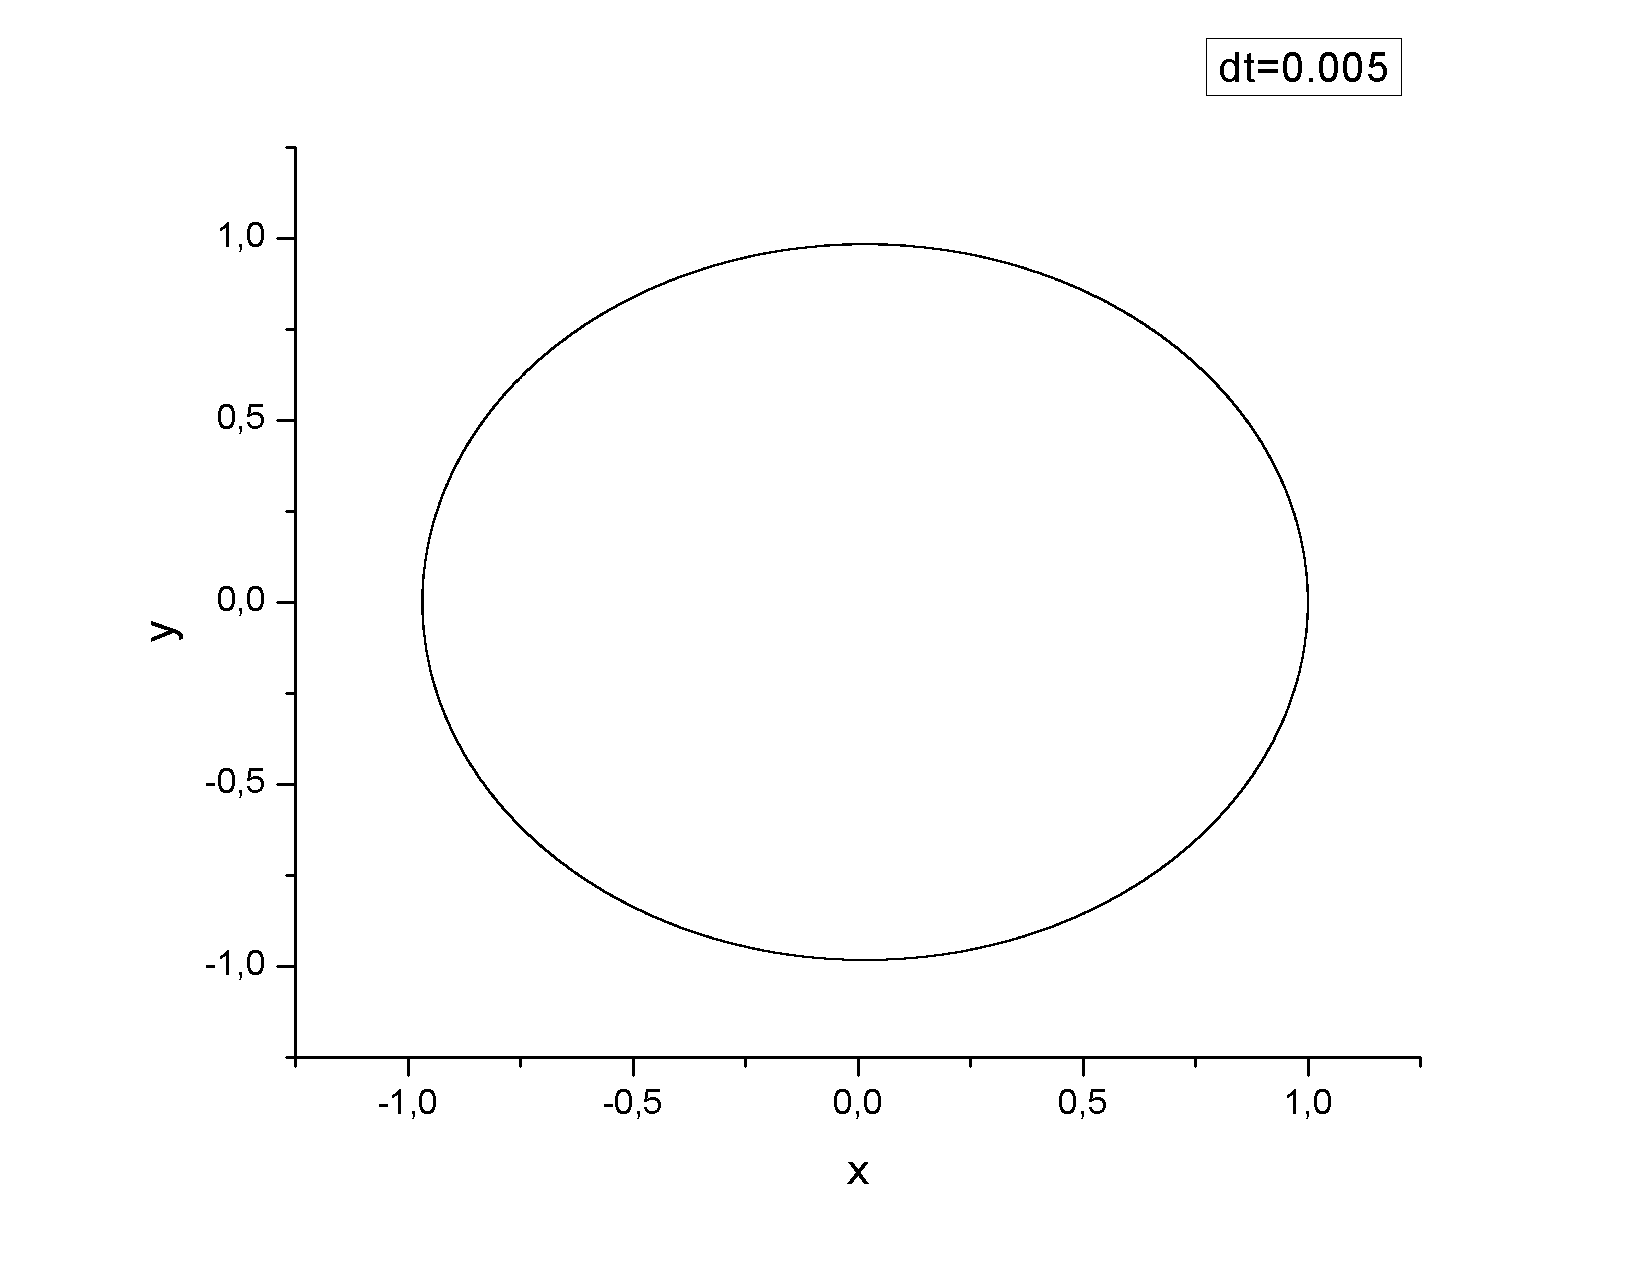
\includegraphics[width=65mm]{f0005} &   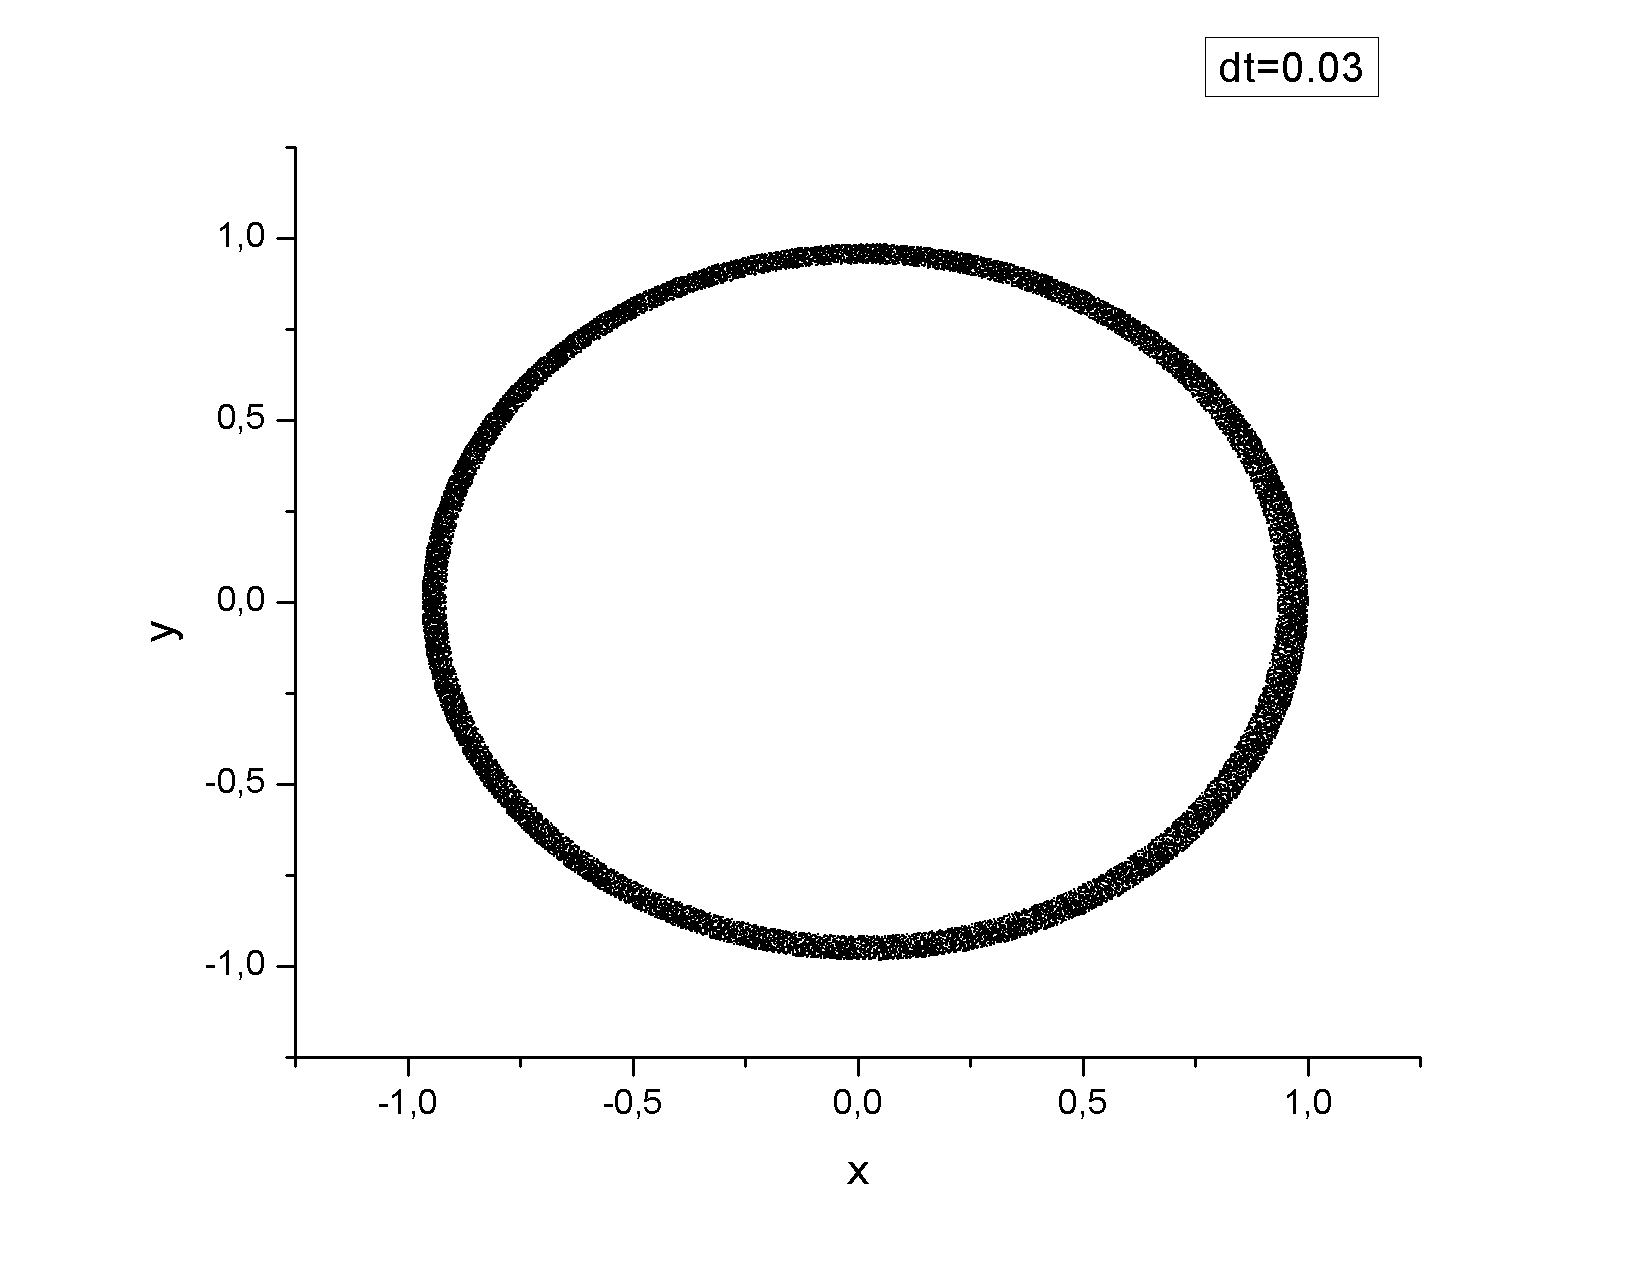
\includegraphics[width=65mm]{f0003} \\
(a) dt=0.005 & (b) dt=0.03 \\[6pt]
 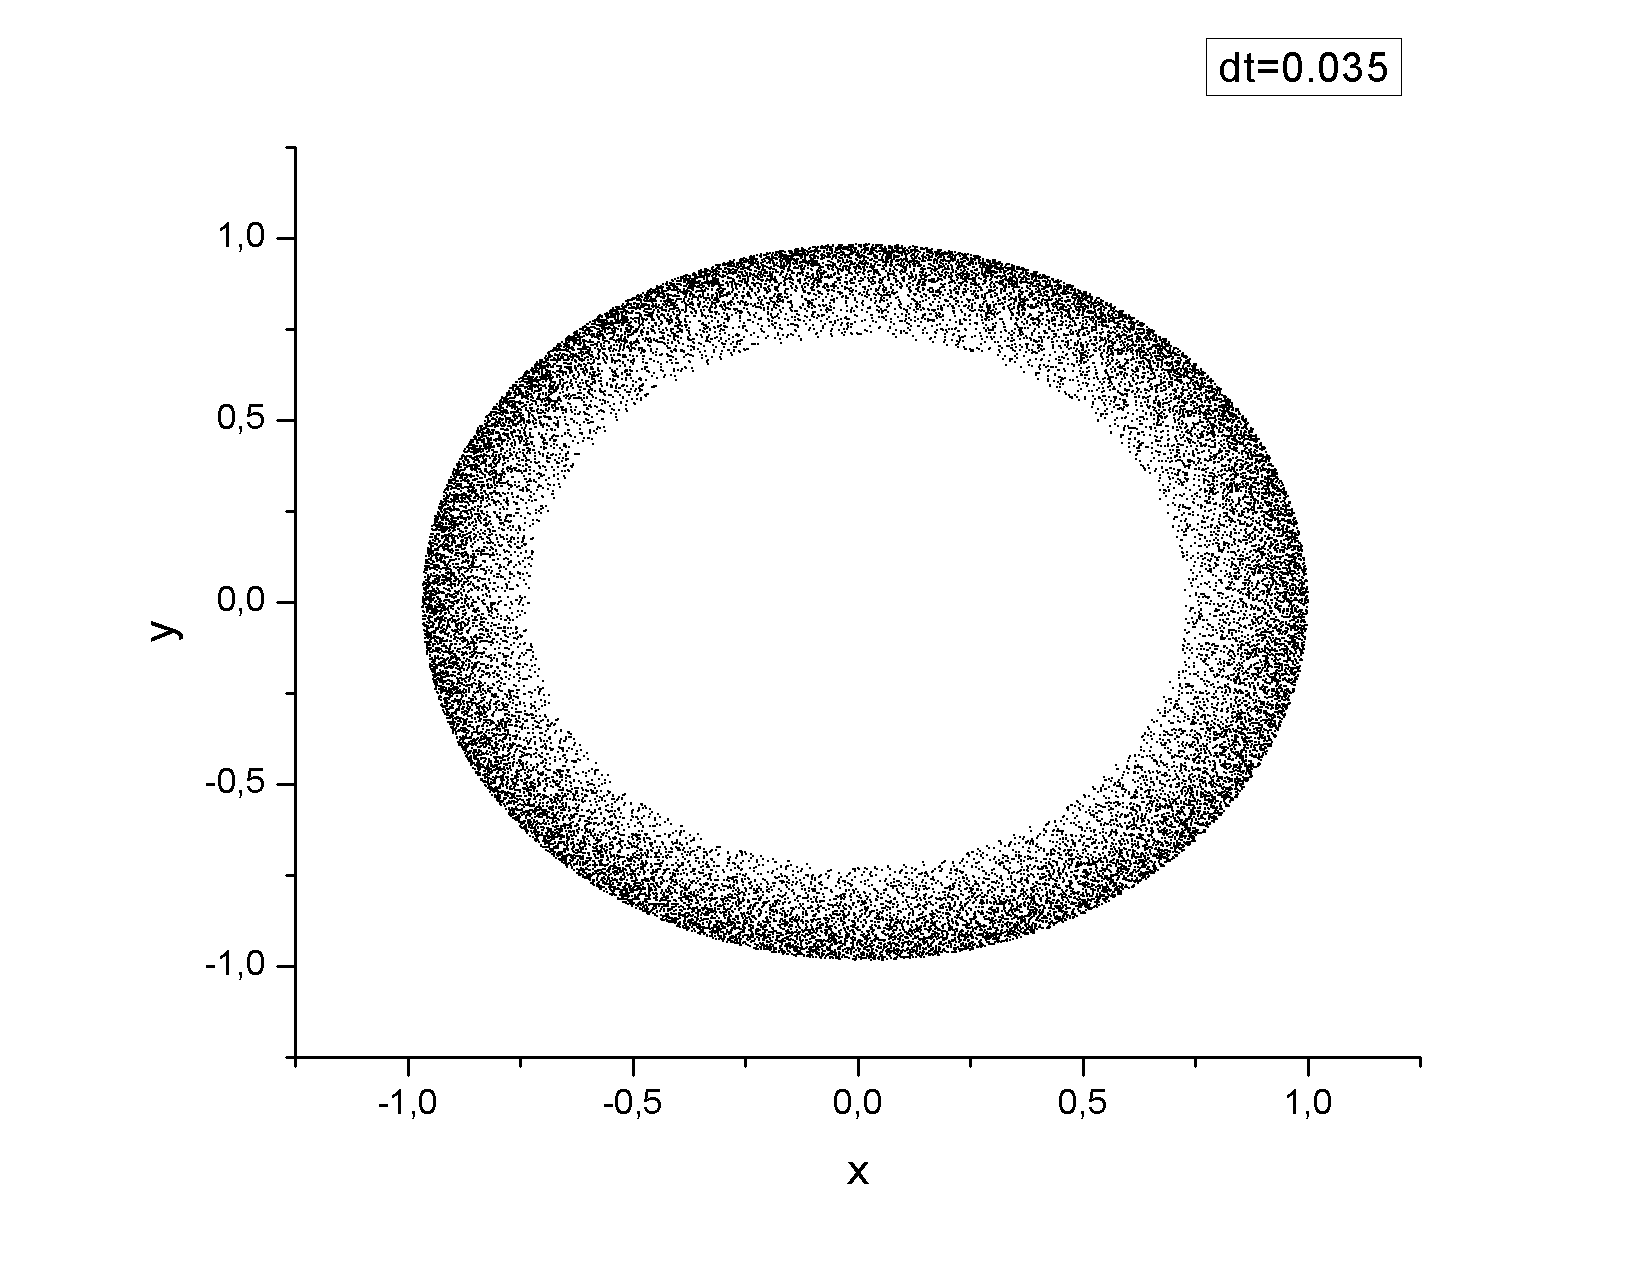
\includegraphics[width=65mm]{f00035} &   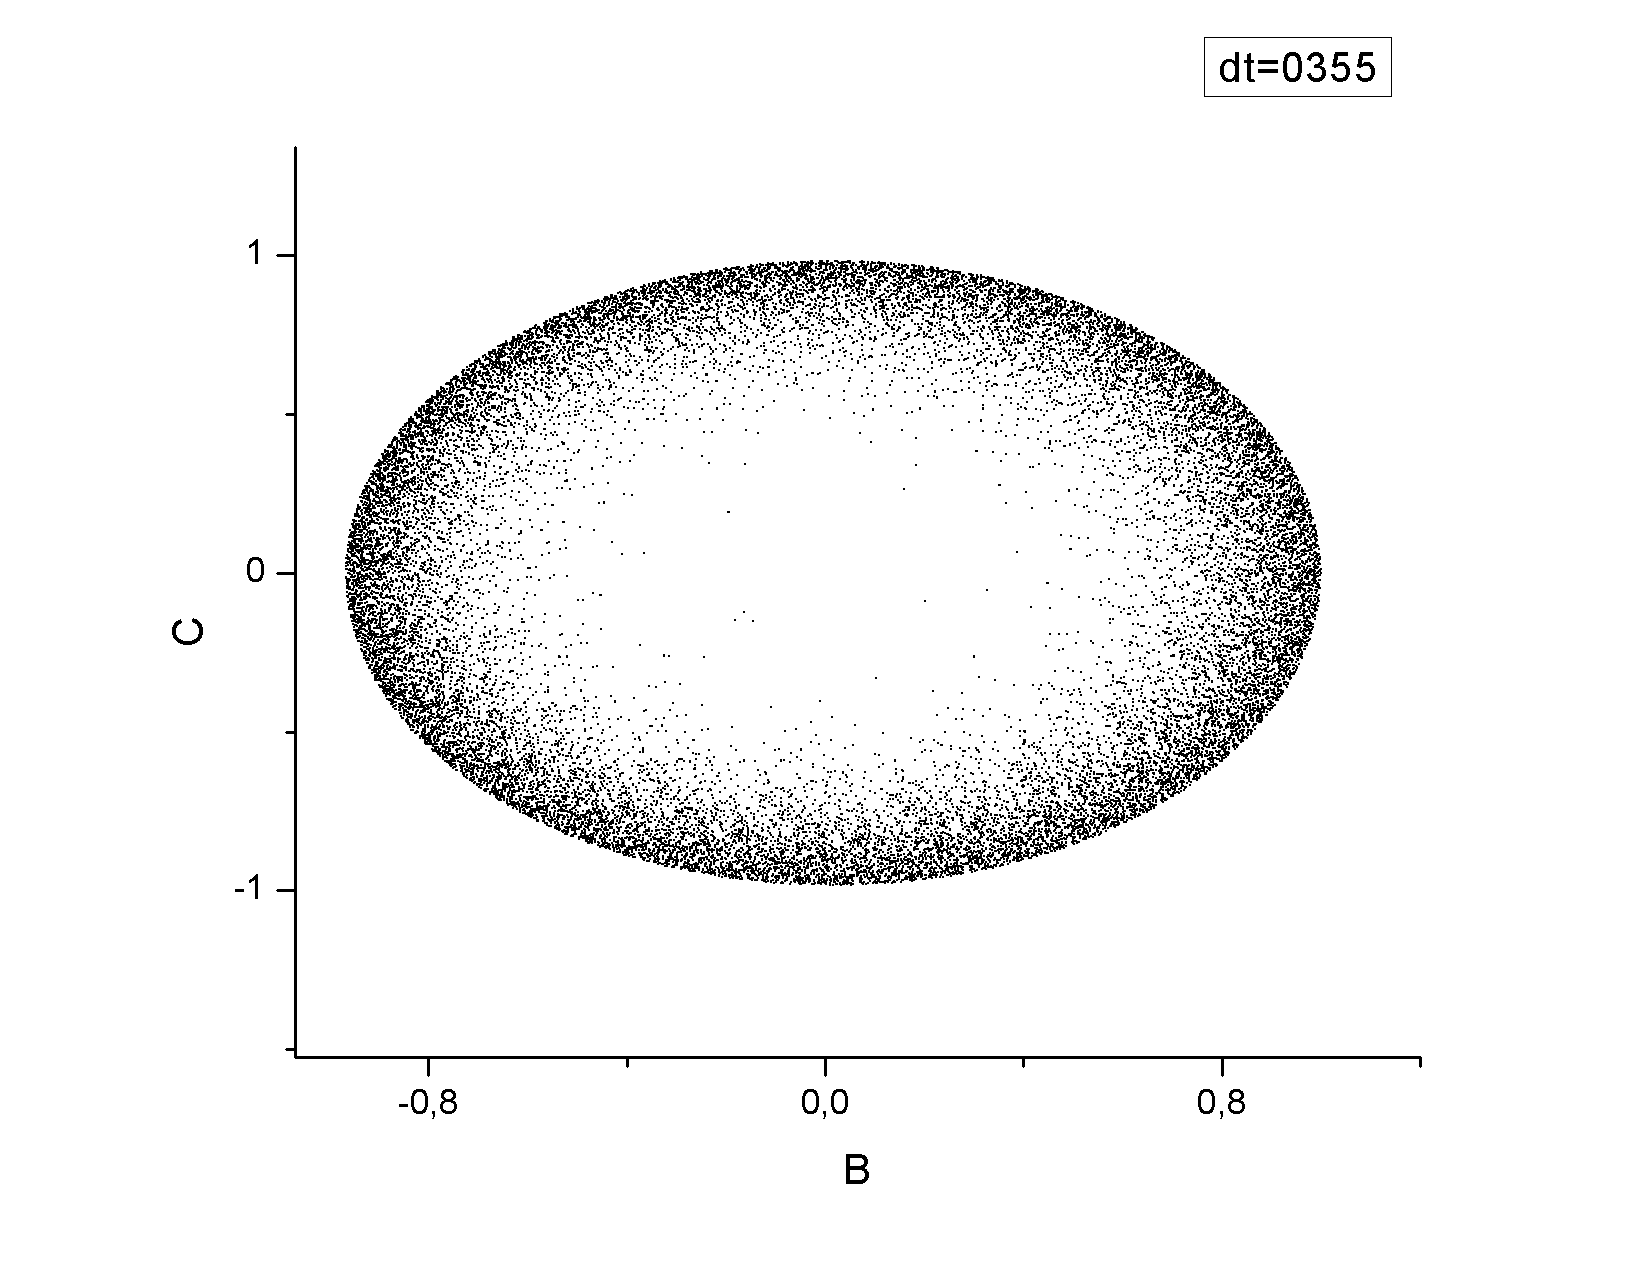
\includegraphics[width=65mm]{f000355} \\
(c) dt=0.035 & (d) dt=0.0355 \\[6pt]
 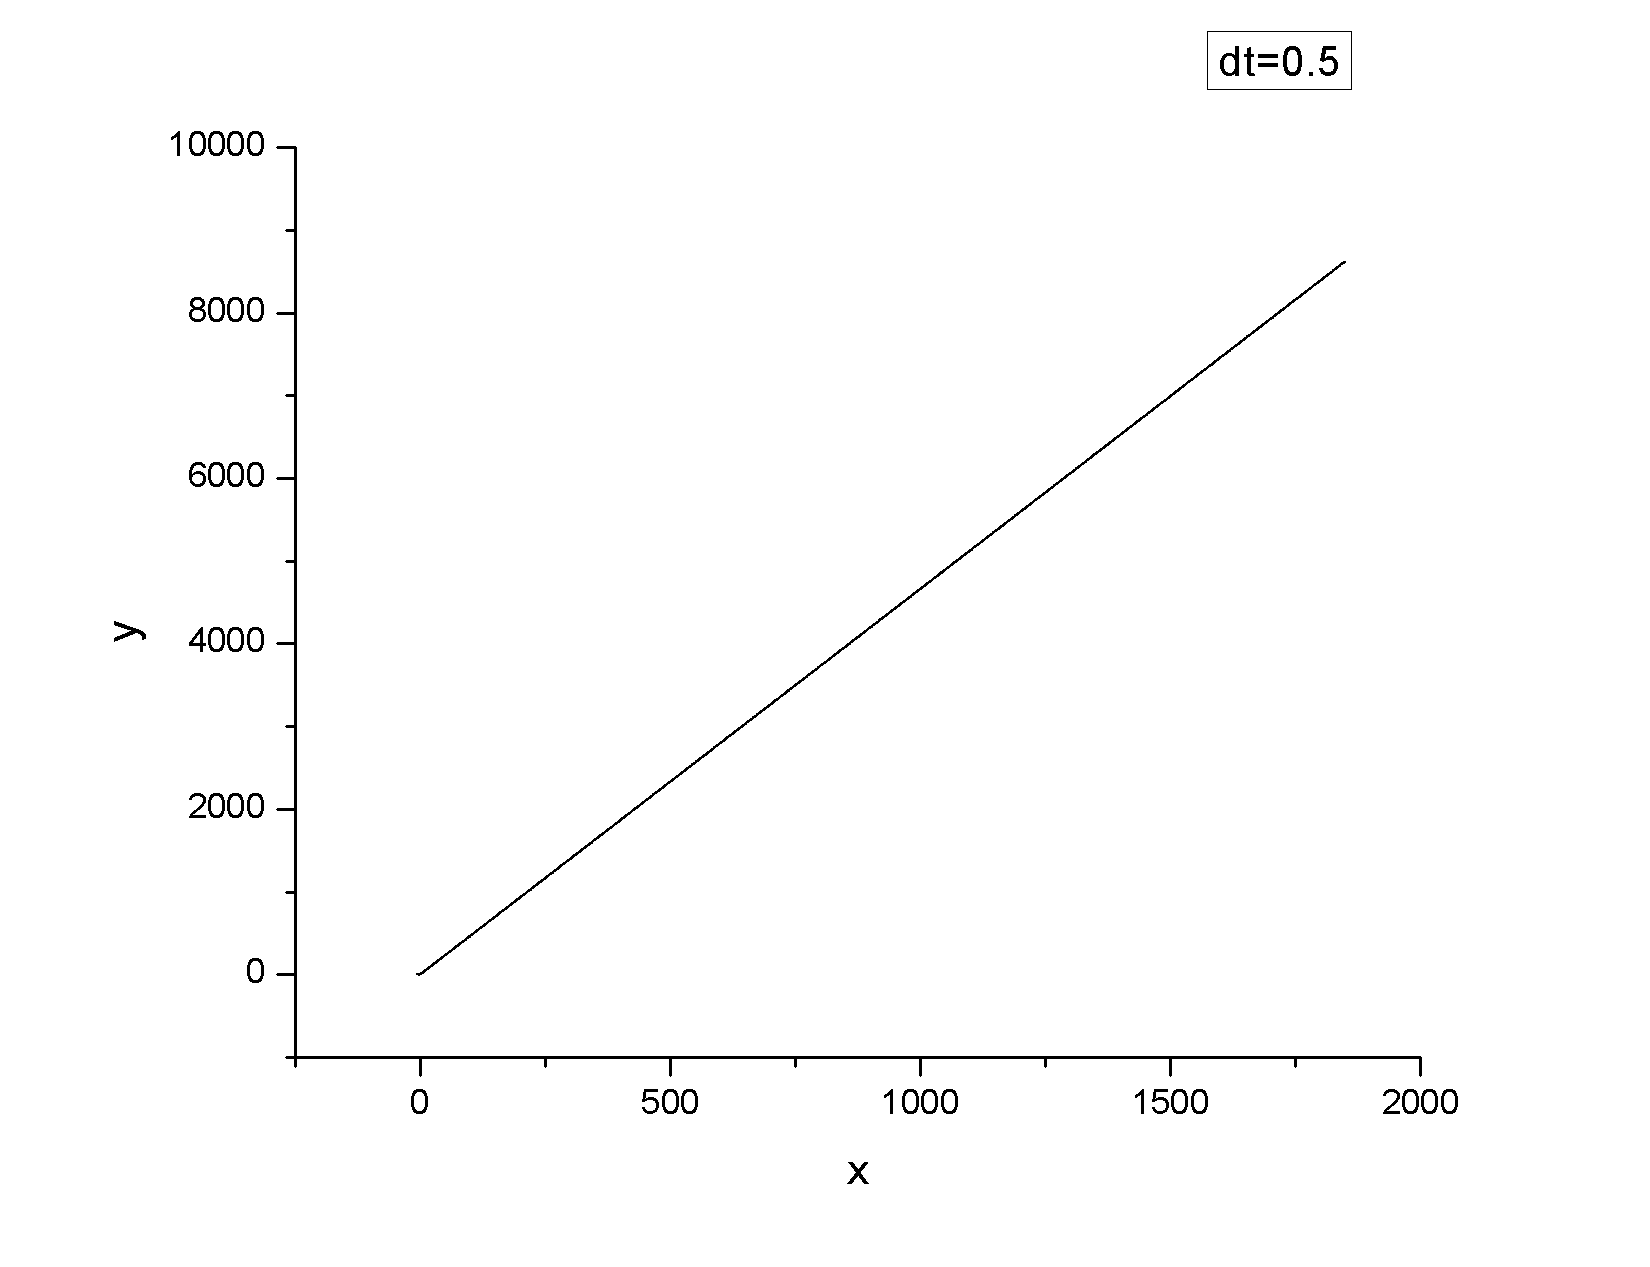
\includegraphics[width=65mm]{f05} &   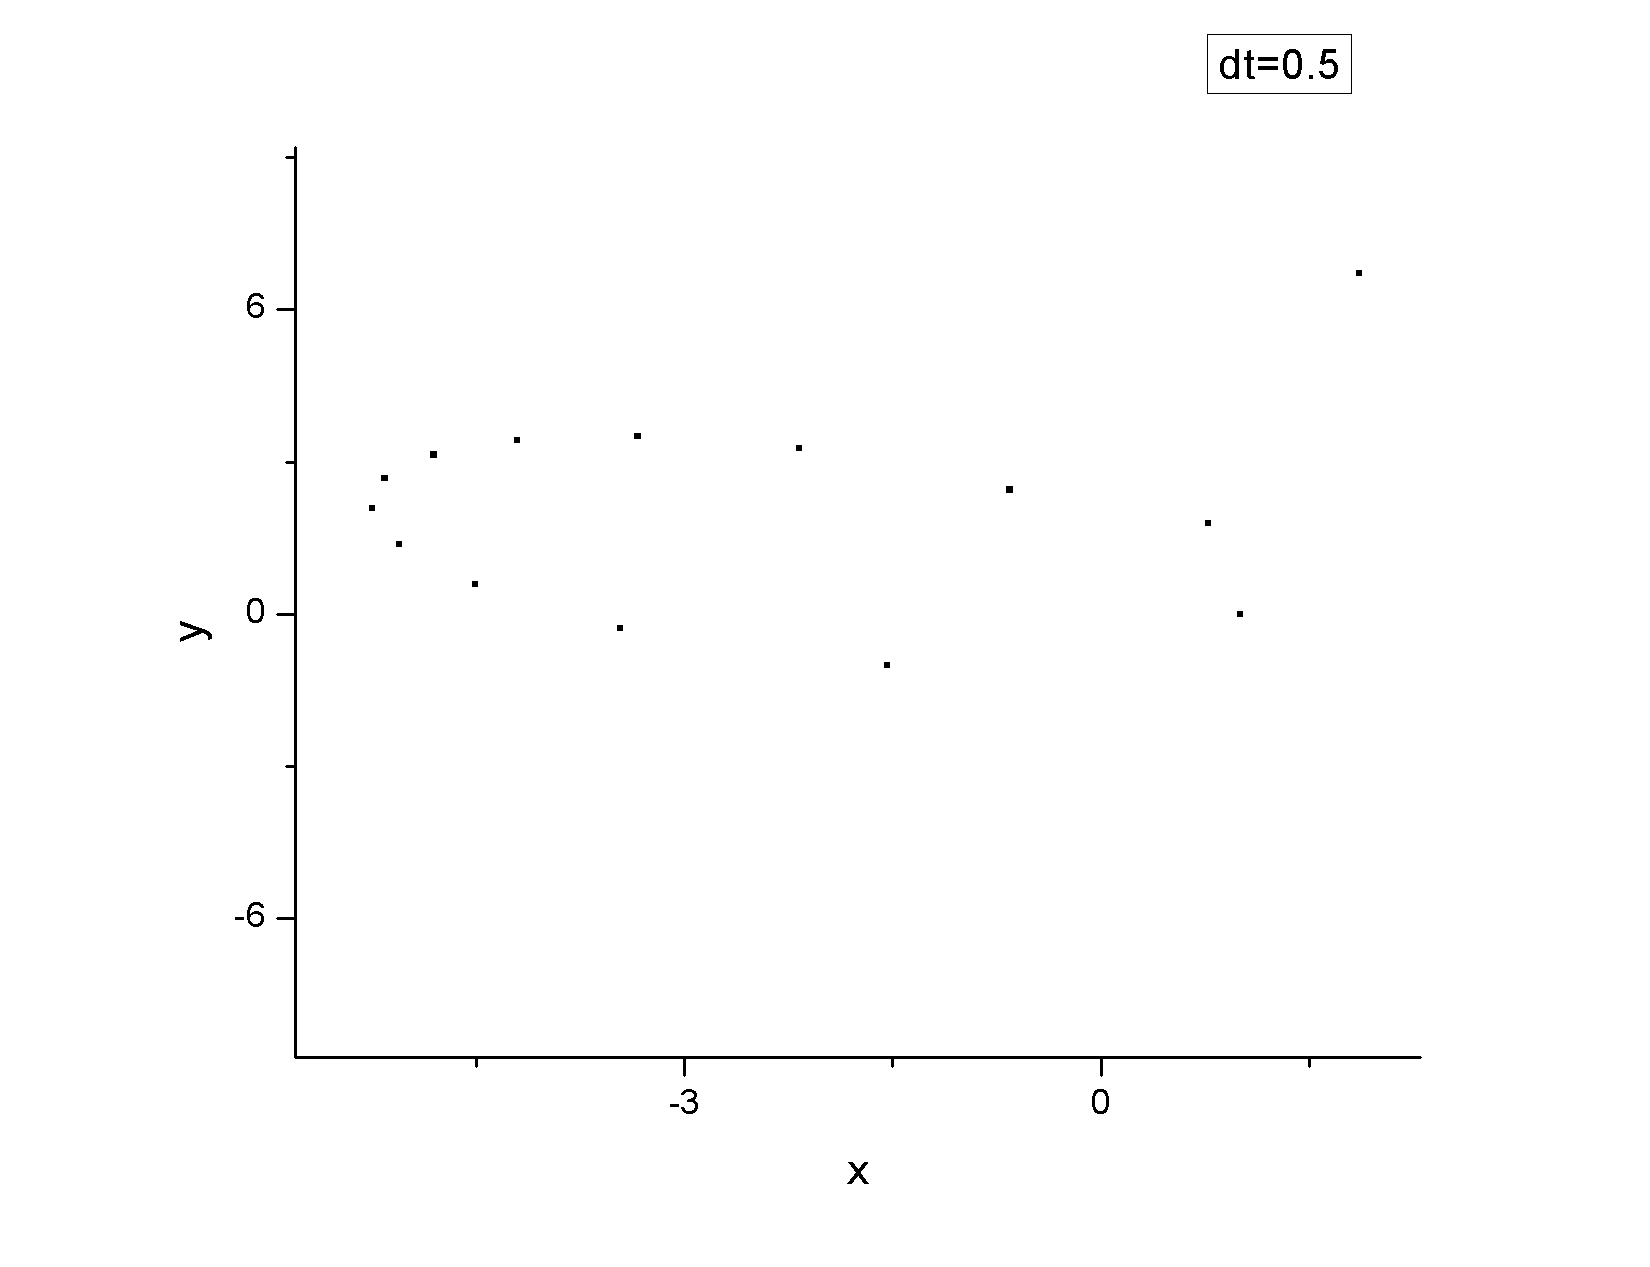
\includegraphics[width=65mm]{f05k} \\
(e) dt=0.5 & (f) dt=0.5 a 0 körül \\[6pt]
\end{tabular}
\caption{A rendszer megváltozása a lépéshosszok modosításval}
\end{figure}

\subsubsection{Az integrálási módszer hatása a nagytengely irányára és méretére}
Ennél a feladatnál azonosan változtattam a lépésközöket, mint az elöző feladatnál, de adaptív lépésközzel integráltam. Ebben az esetben is megvizsgáltam az összes lépésközre a problémát, de mivel lényegi változást nem produkált a pálya alakja ennél az integrálási technikánál így csak a legkisebb valamint a legnagyobb lépésközre vizsgált esetet mutatom be.

\begin{figure}[H]
\begin{tabular}{cc}
  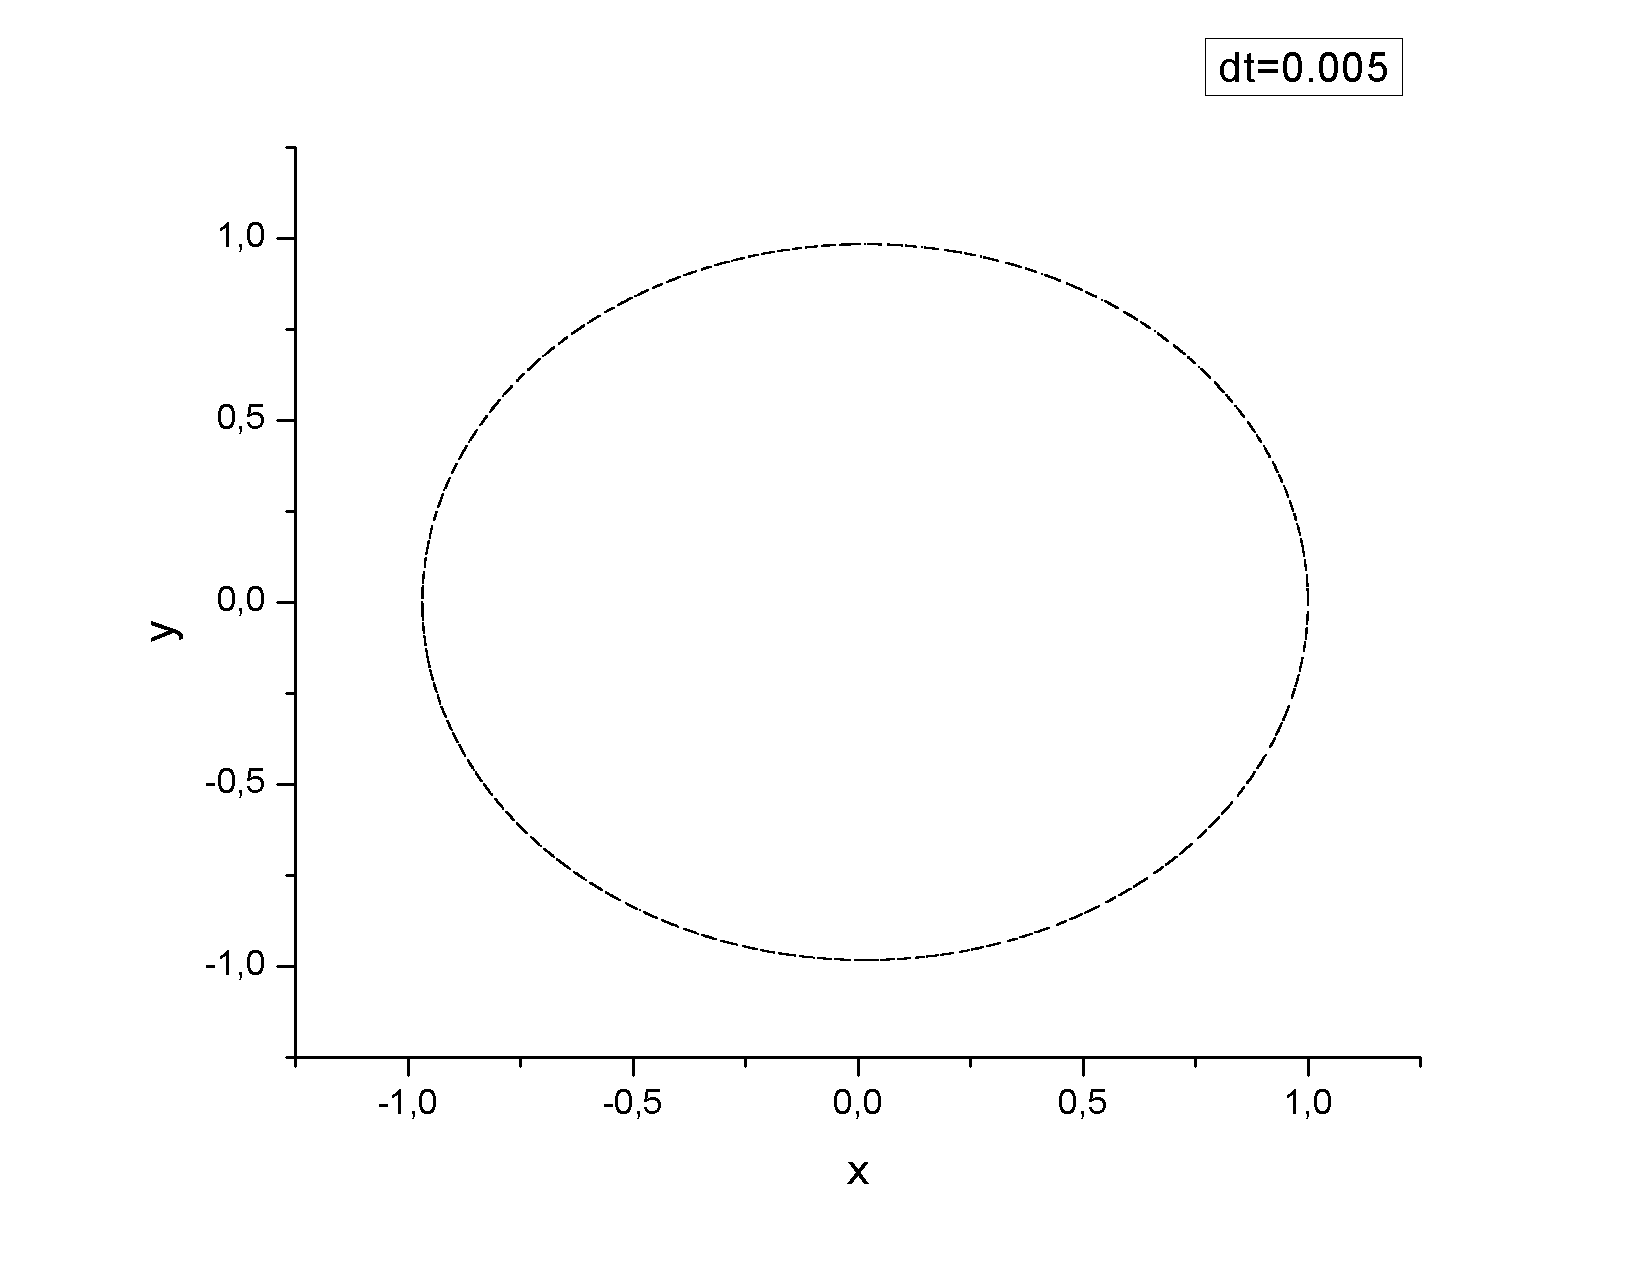
\includegraphics[width=65mm]{a0005} &   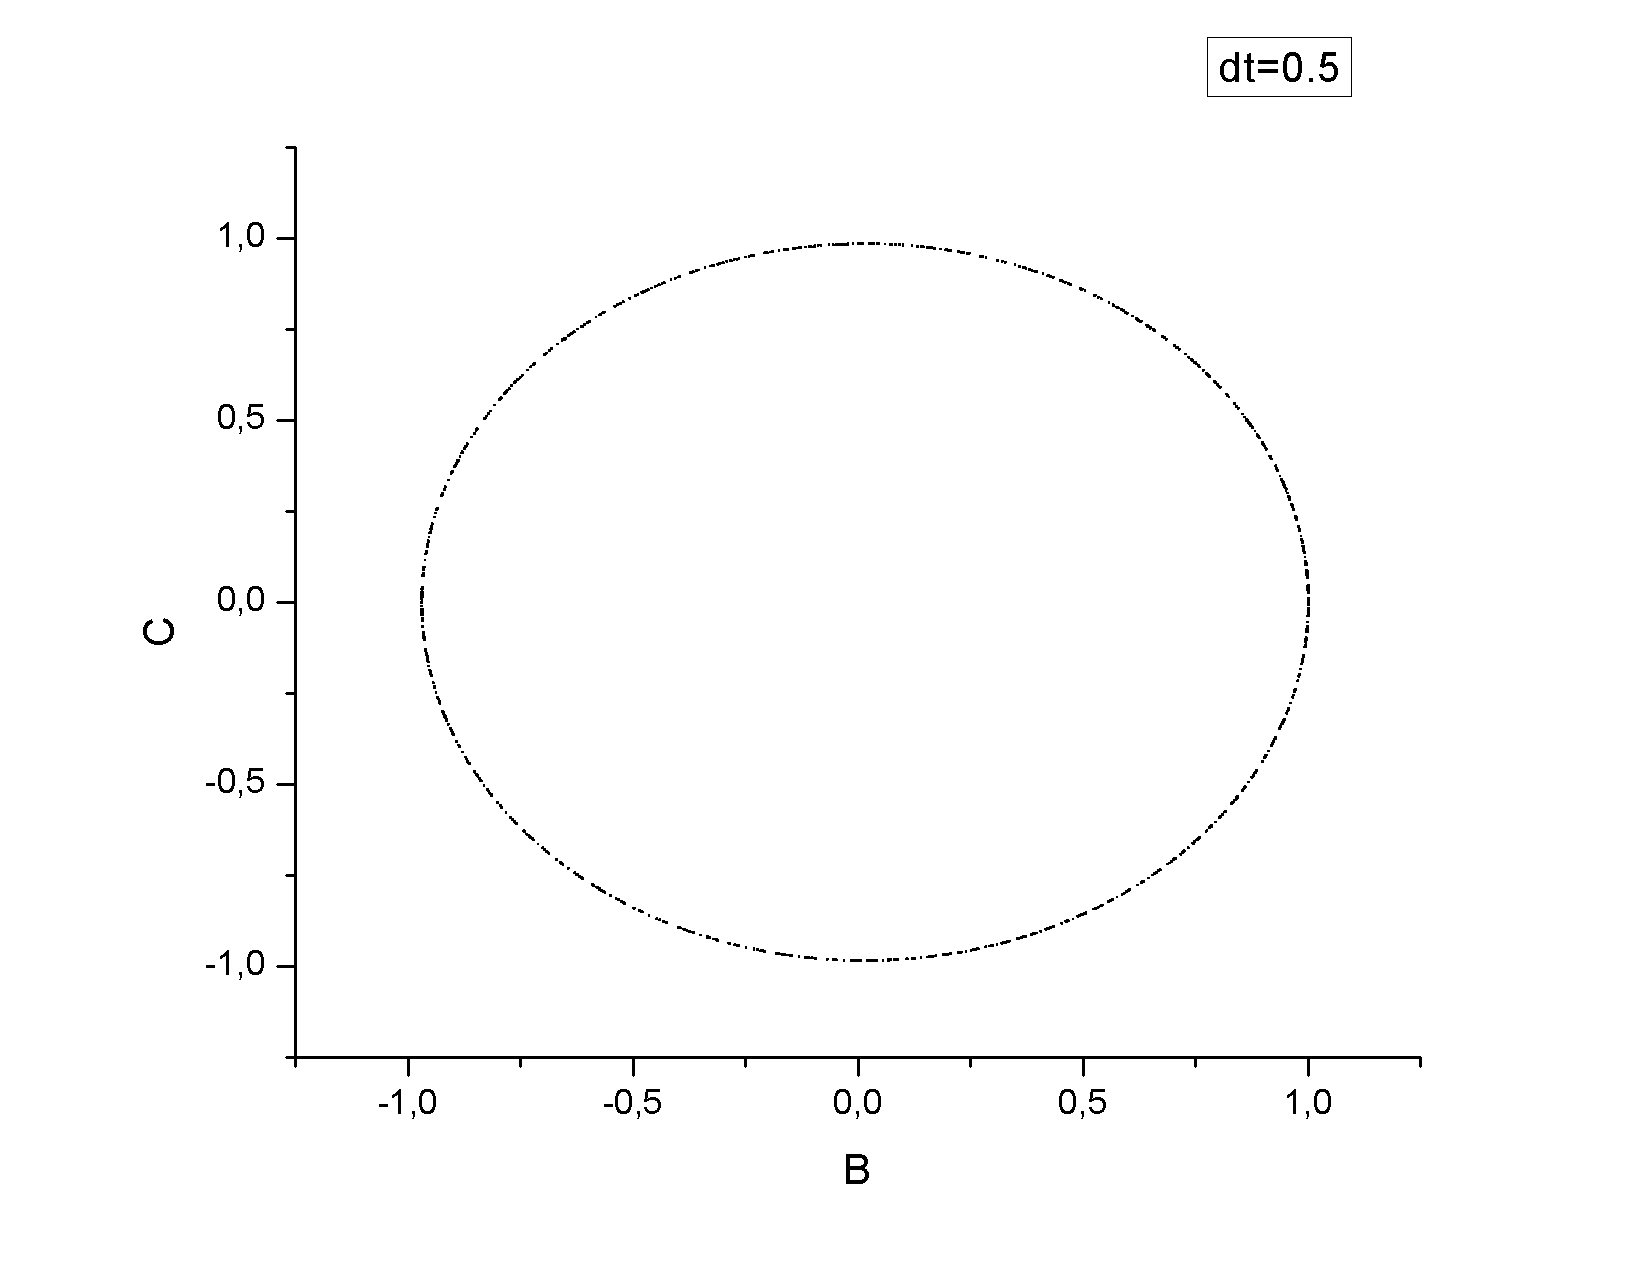
\includegraphics[width=65mm]{a05} \\
(a) dt=0.005 & (b) dt=0.5 
\end{tabular}
\caption{A rendszer megváltozása a lépéshosszok modosításval és adaptív lépésközzel}
\end{figure}


\subsection{Adaptív lépéshossz változása a pálya mentén}
Ennél a feladatnál azt vizsgáltam, hogy a lépéshossz abban az esetben amikor adaptívan változik, milyen mértékben teszi ezt és hol.

\begin{figure}[H]
  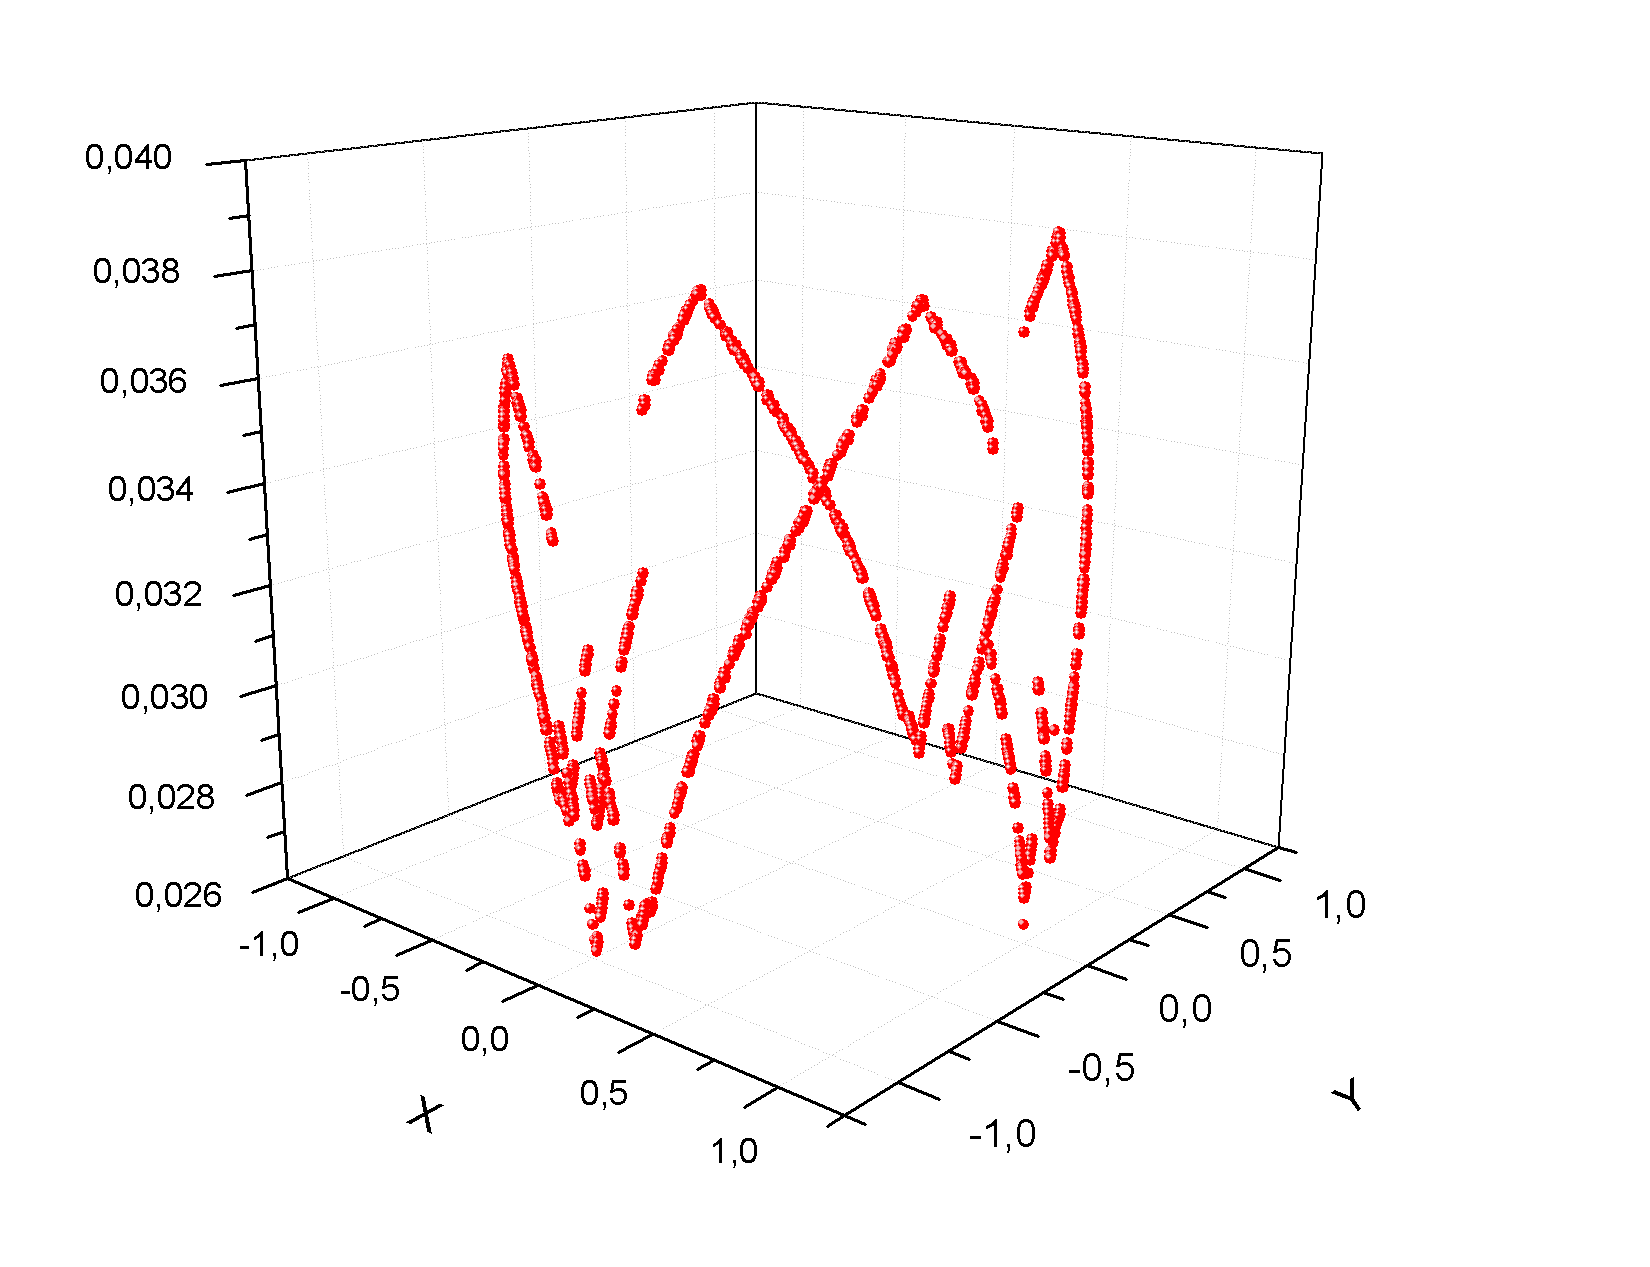
\includegraphics[width=\textwidth]{lepes}
\caption{Az lépéshosszok változása a pálya mentén}
\end{figure}
Azt figyelhettük meg az első kettő mérési feladatban, hogy a lépés szám nagyban befolyásolja a fix lépésközös integrálást, mivel hirtelen változásoknál könnyen elöfordulhat, hogy nem vételez elég mintát és így a mi esetünkben például a bolygók elfognak repülni. Az adaptív lépésközös módszert ez a probléma nem érintette, mivel ahol nagyobb mértékü változás történt ott besürüsödött a lépések száma és ez véget hiába választottam nagy lépés közt a program ahol érzékelte, hogy nagy mértékű változás történik ott besűrűsítette a lépések számát. 

\subsection{Merkúr perihélium processziója}
A Merkúr pályájának az elfordulása az általános relativítás elmélet ad magyarázatot. 
\begin{itemize}
  \item aphélium távolság: 0.466 AU
  \item excentricitás:0.2056
  \item periodus szám: 1000
  \item adaptív pontosság: 0.00001
\end{itemize}

Így a következő képpen kell átalakítani a szimuláció egyenletét:

\begin{align}
F_{12}=-G\frac{m_1m_2}{r_{12}^2}(1+\frac{a}{r^2})
\end{align}
Ezt a program kódban a következő képpen írtam be:
\newline
$f[3] = - GmPlusM * r _ x / rCubed*(1 + (1.1e-8/rSquared));$
\newline
$f[4] = - GmPlusM *  r _ y / rCubed*(1 + (1.1e-8/rSquared));$
 \newline


A precesszió megfigyelhető a pályénak a két dimenziós ábráján is a vonalak kiszélesedésén is keresztül.
\begin{figure}[H]
  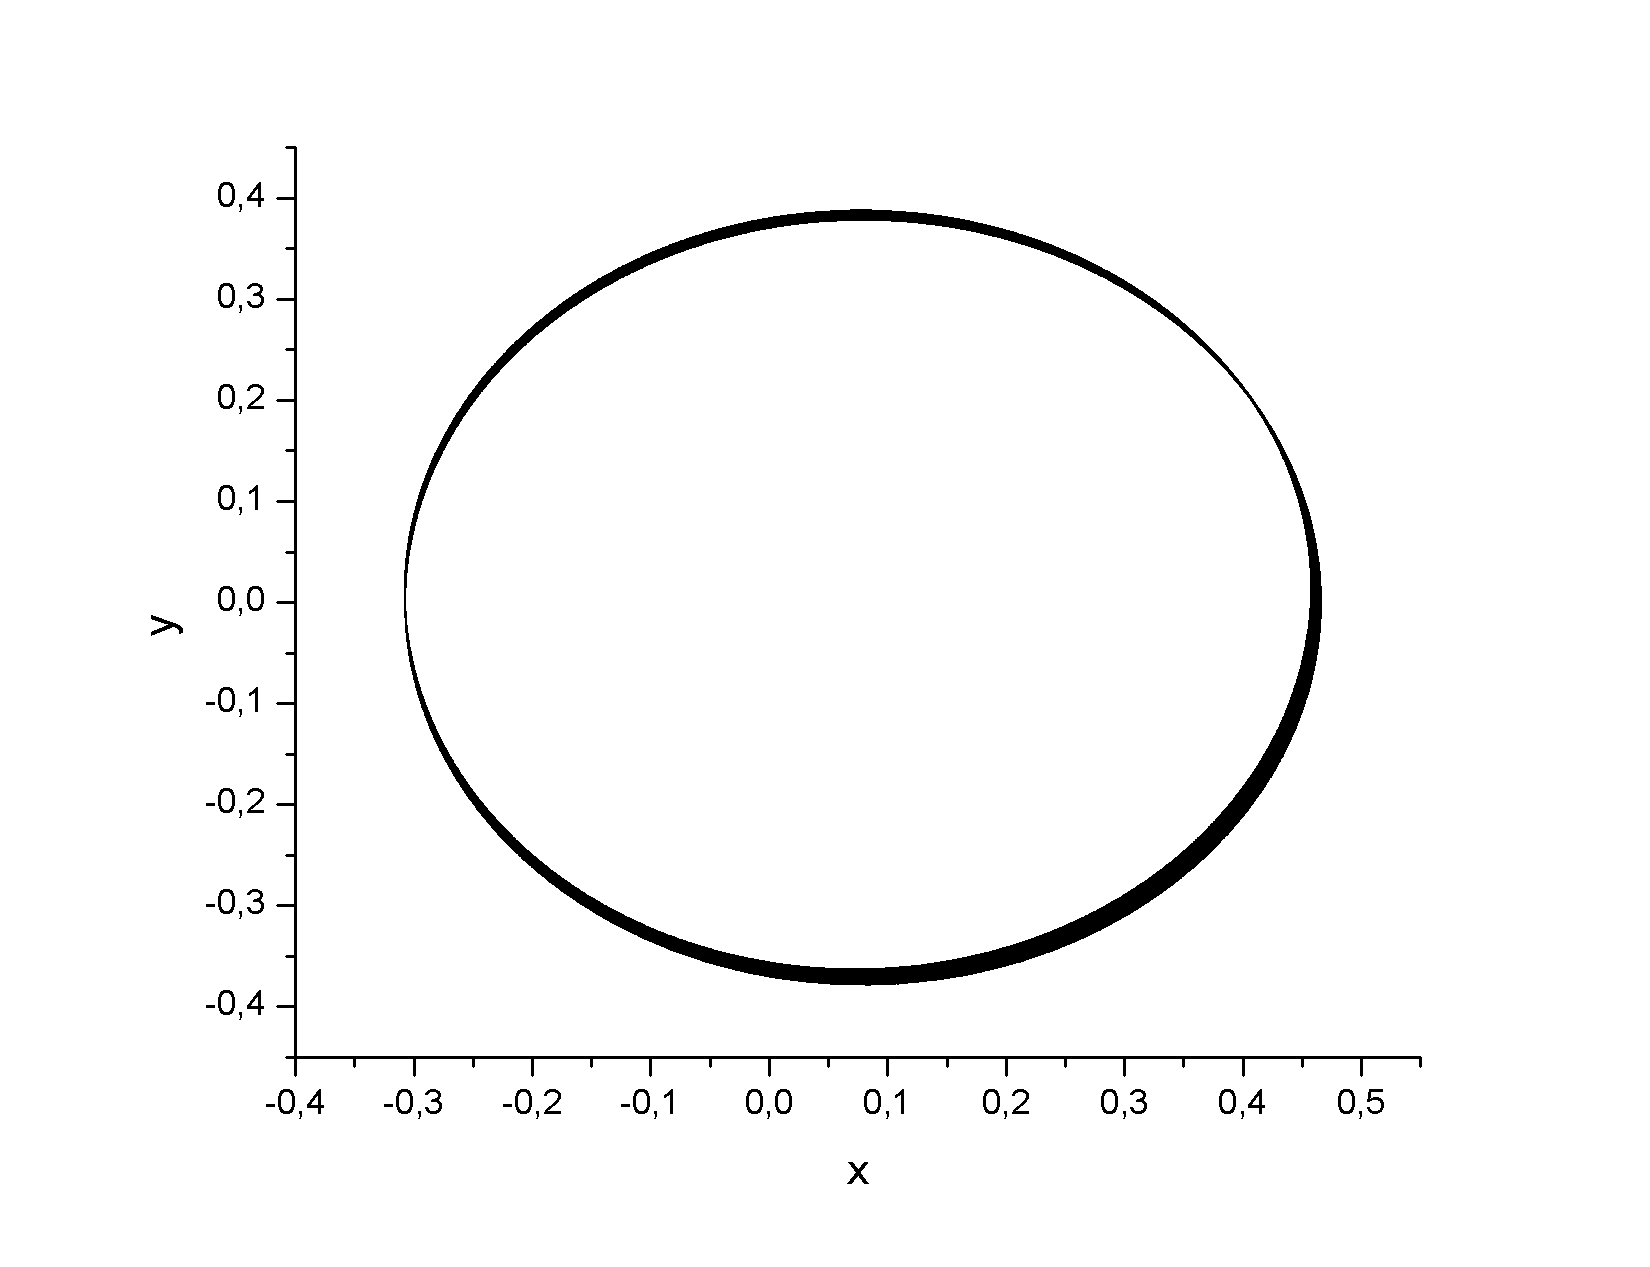
\includegraphics[width=\textwidth]{merkur}
\caption{A Merkúr precessziója}
\end{figure}

Szemléletesebben a következő ábrán láthatjuk a jelenséget ahol a naptól vett távolságot ábrázoltam a helytől függően.
\begin{figure}[H]
  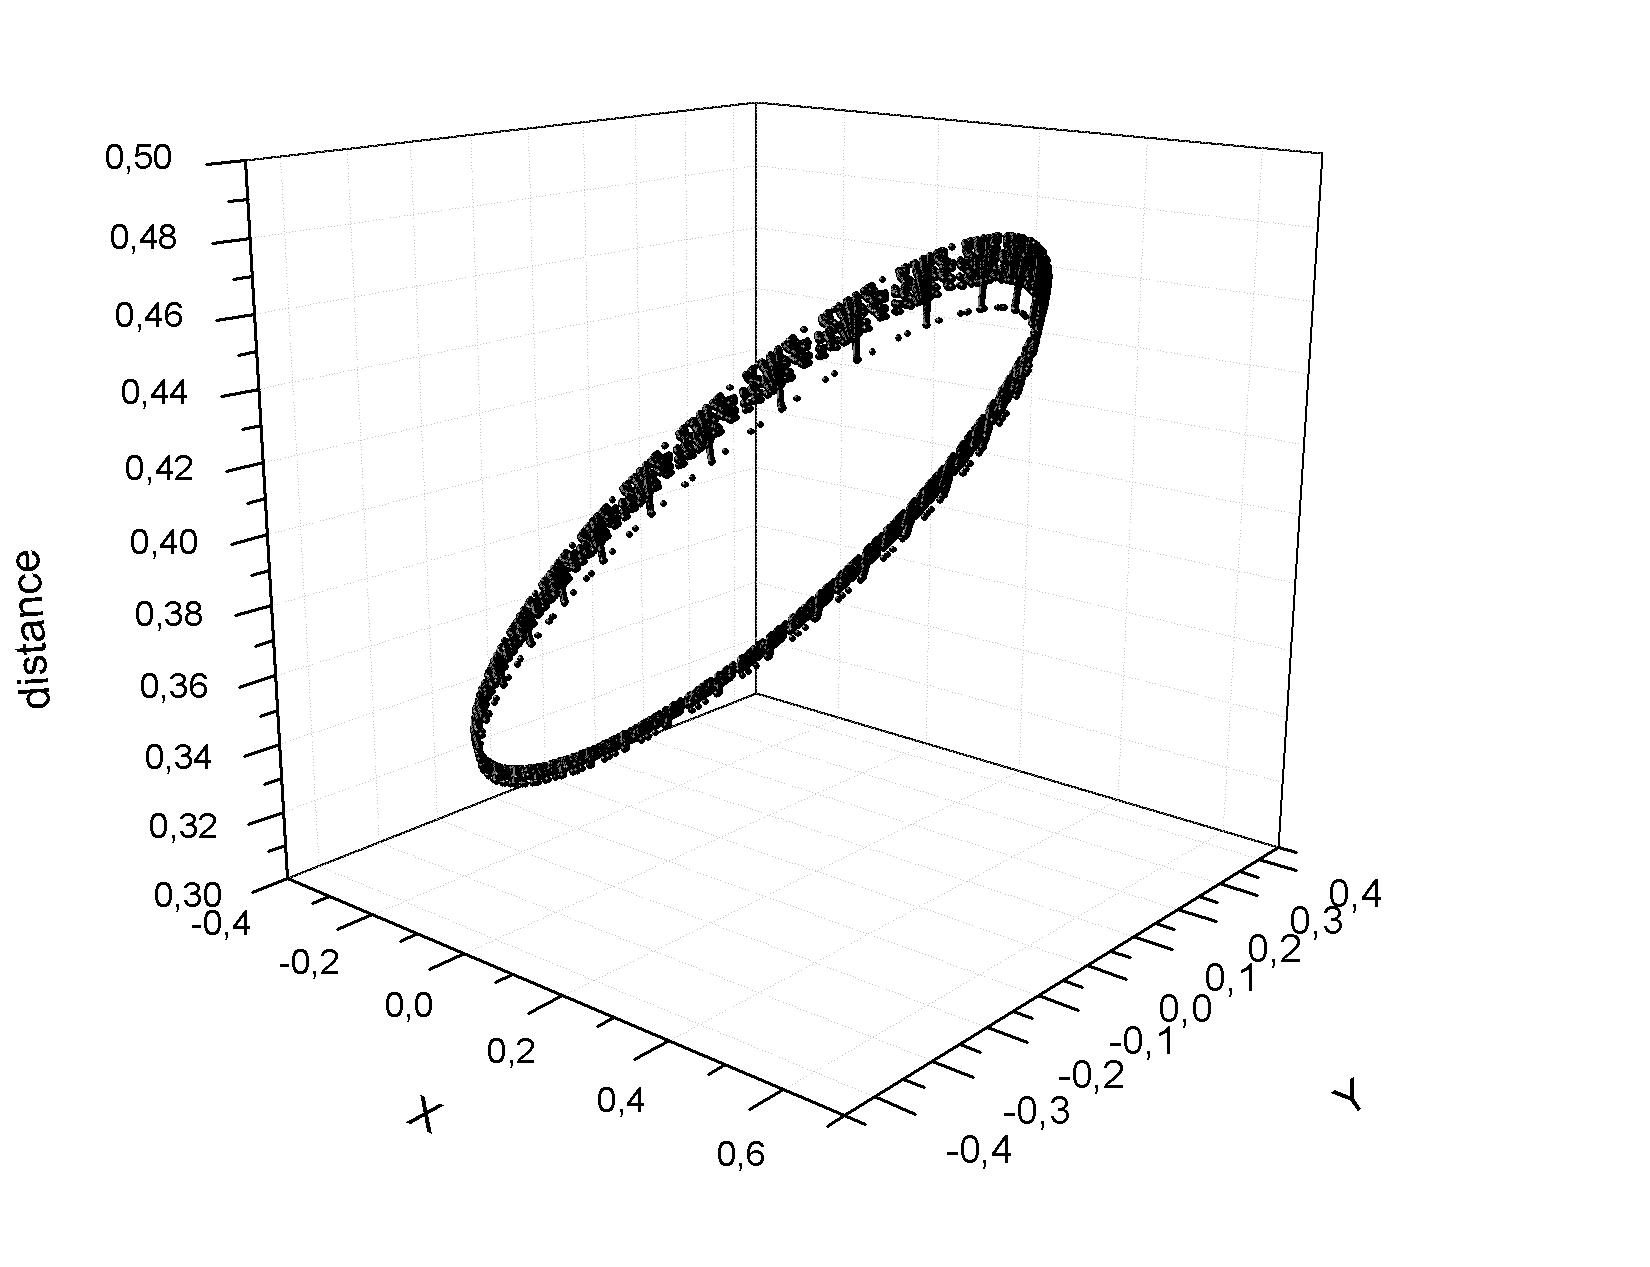
\includegraphics[width=\textwidth]{merkur3d}
\caption{A Merkúr pályájának a függvényében a távolsága a naptól}
\end{figure}





\subsection{Háromtest probléma}
Ebben a feladatban a Jupitert és a Földet közösen probáltam meg szimulálni a naprendszerben.
\newline
A következő differenciál egyenletekkel írhatjuk le a rendszert:

\begin{align}
&\ddot{x_1}=-Gm_2\frac{x_1-x_2}{|x_1-x_2|^3}-Gm_3\frac{x_1-x_3}{|x_1-x_3|^3}\\
&\ddot{x_2}=-Gm_3\frac{x_2-x_3}{|x_2-x_3|^3}-Gm_1\frac{x_2-x_1}{|x_2-x_1|^3}\\
&\ddot{x_3}=-Gm_1\frac{x_3-x_1}{|x_3-x_1|^3}-Gm_2\frac{x_3-x_2}{|x_3-x_2|^3}\\
\end{align}

A rendszer egyszerübbé tételéhez tételezzük fel hogy a nap tömege annyival nagyobb a Jupite és a Föld tömegénél, hogy fix pontként tekinthetjük ami körül fog keringeni a másik két test. 
\newline
A Jupiter adatai:
\begin{itemize}
  \item aphélium távolság: 5,5 AU
  \item excentricitás:0.05
  \item tömeg a föld tömegének számszorosával kifejezve: 318
\end{itemize}

\begin{figure}[H]
  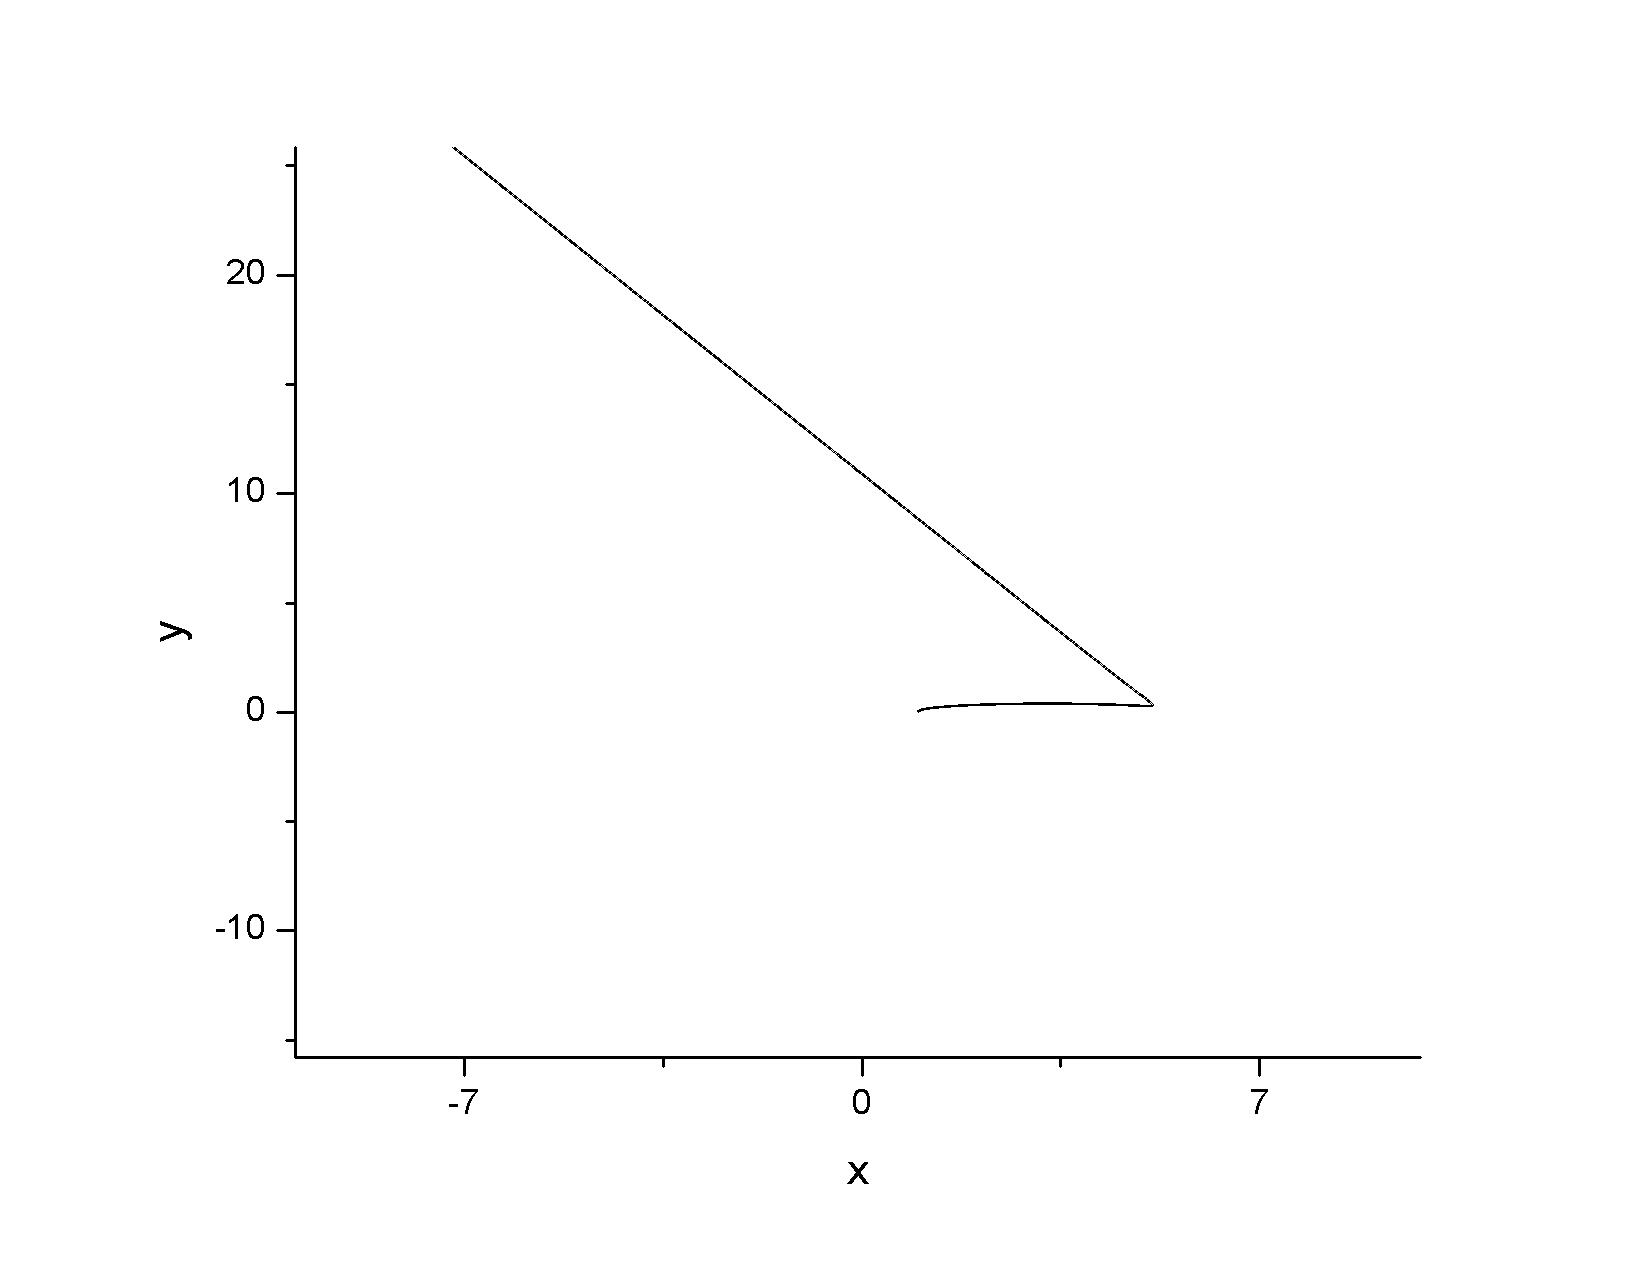
\includegraphics[width=0.75\textwidth]{3}
\caption{A Föld pályája a Jupiter jelenlétében}
\end{figure}

\begin{figure}[H]
  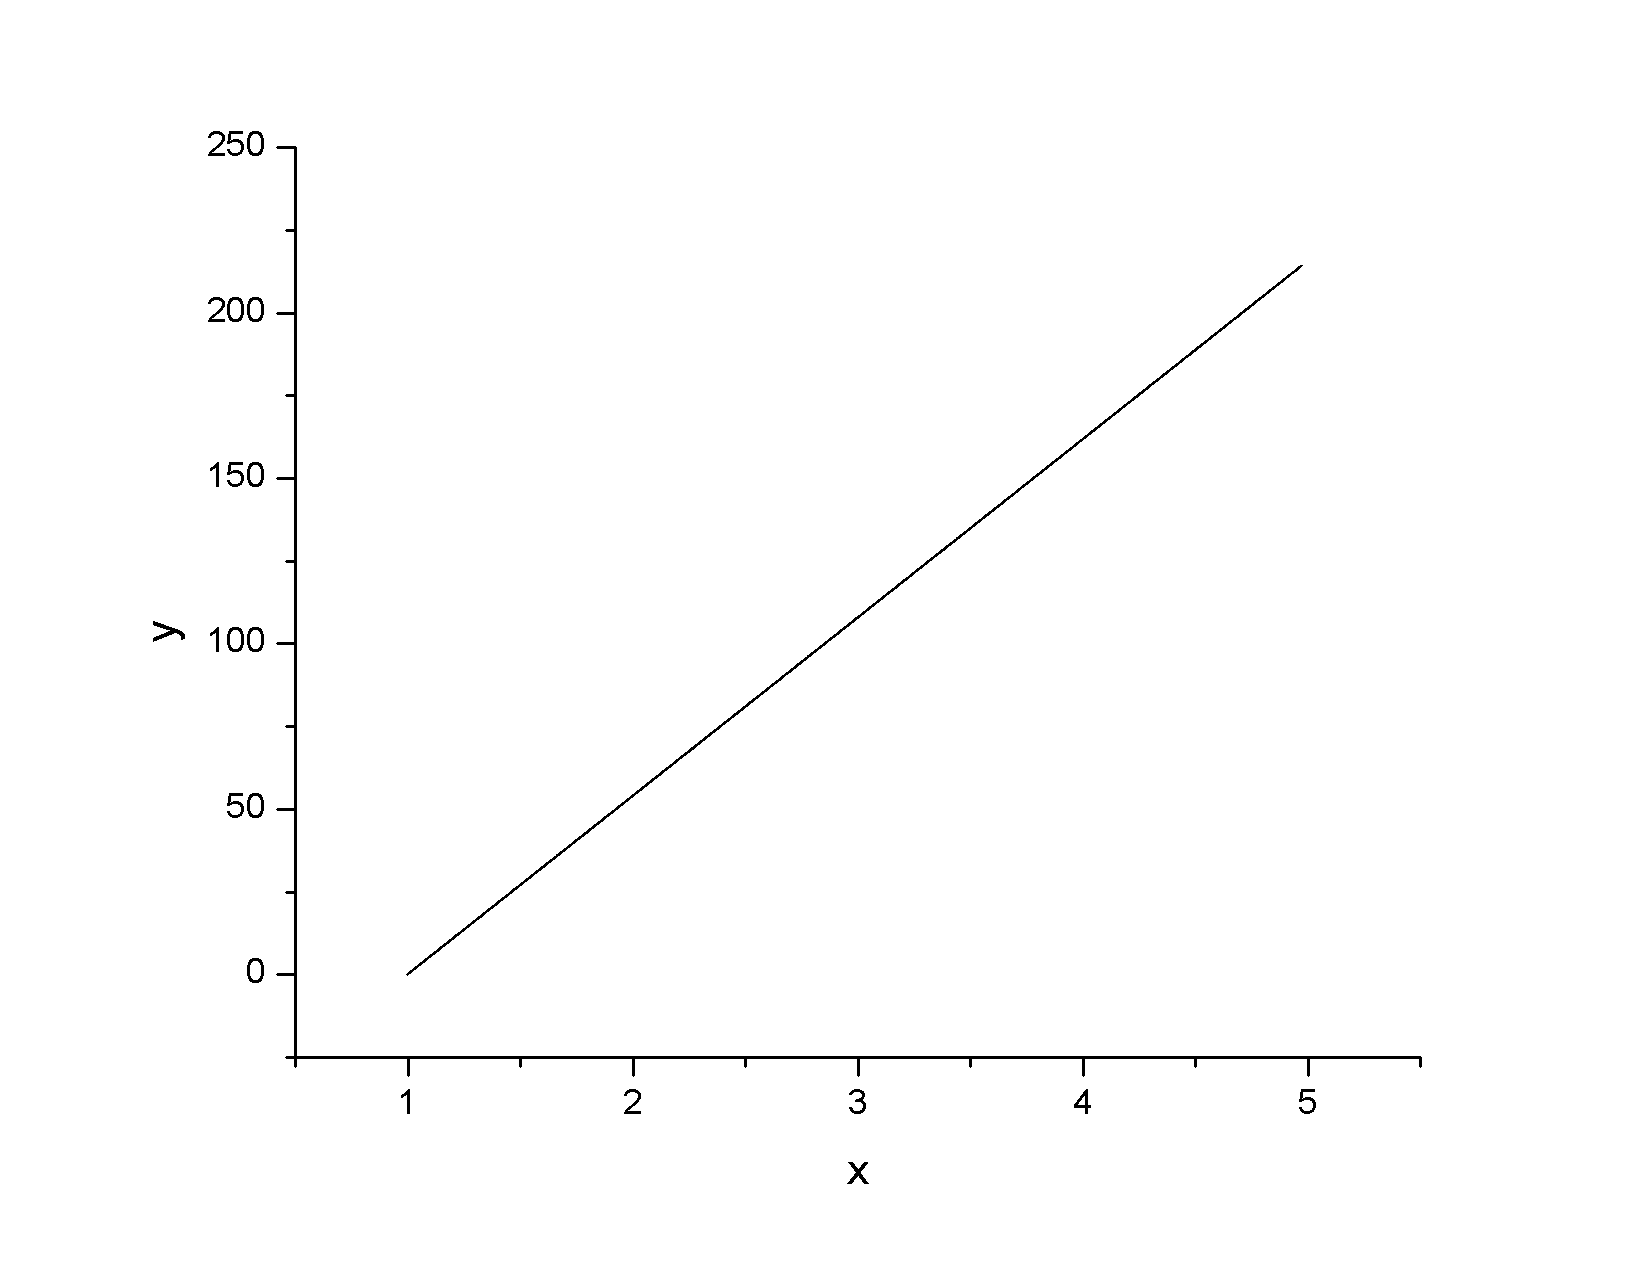
\includegraphics[width=0.75\textwidth]{3testjupiter}
\caption{A Jupiter pályája a Föld jelenlétében}
\end{figure}

\begin{figure}[H]
  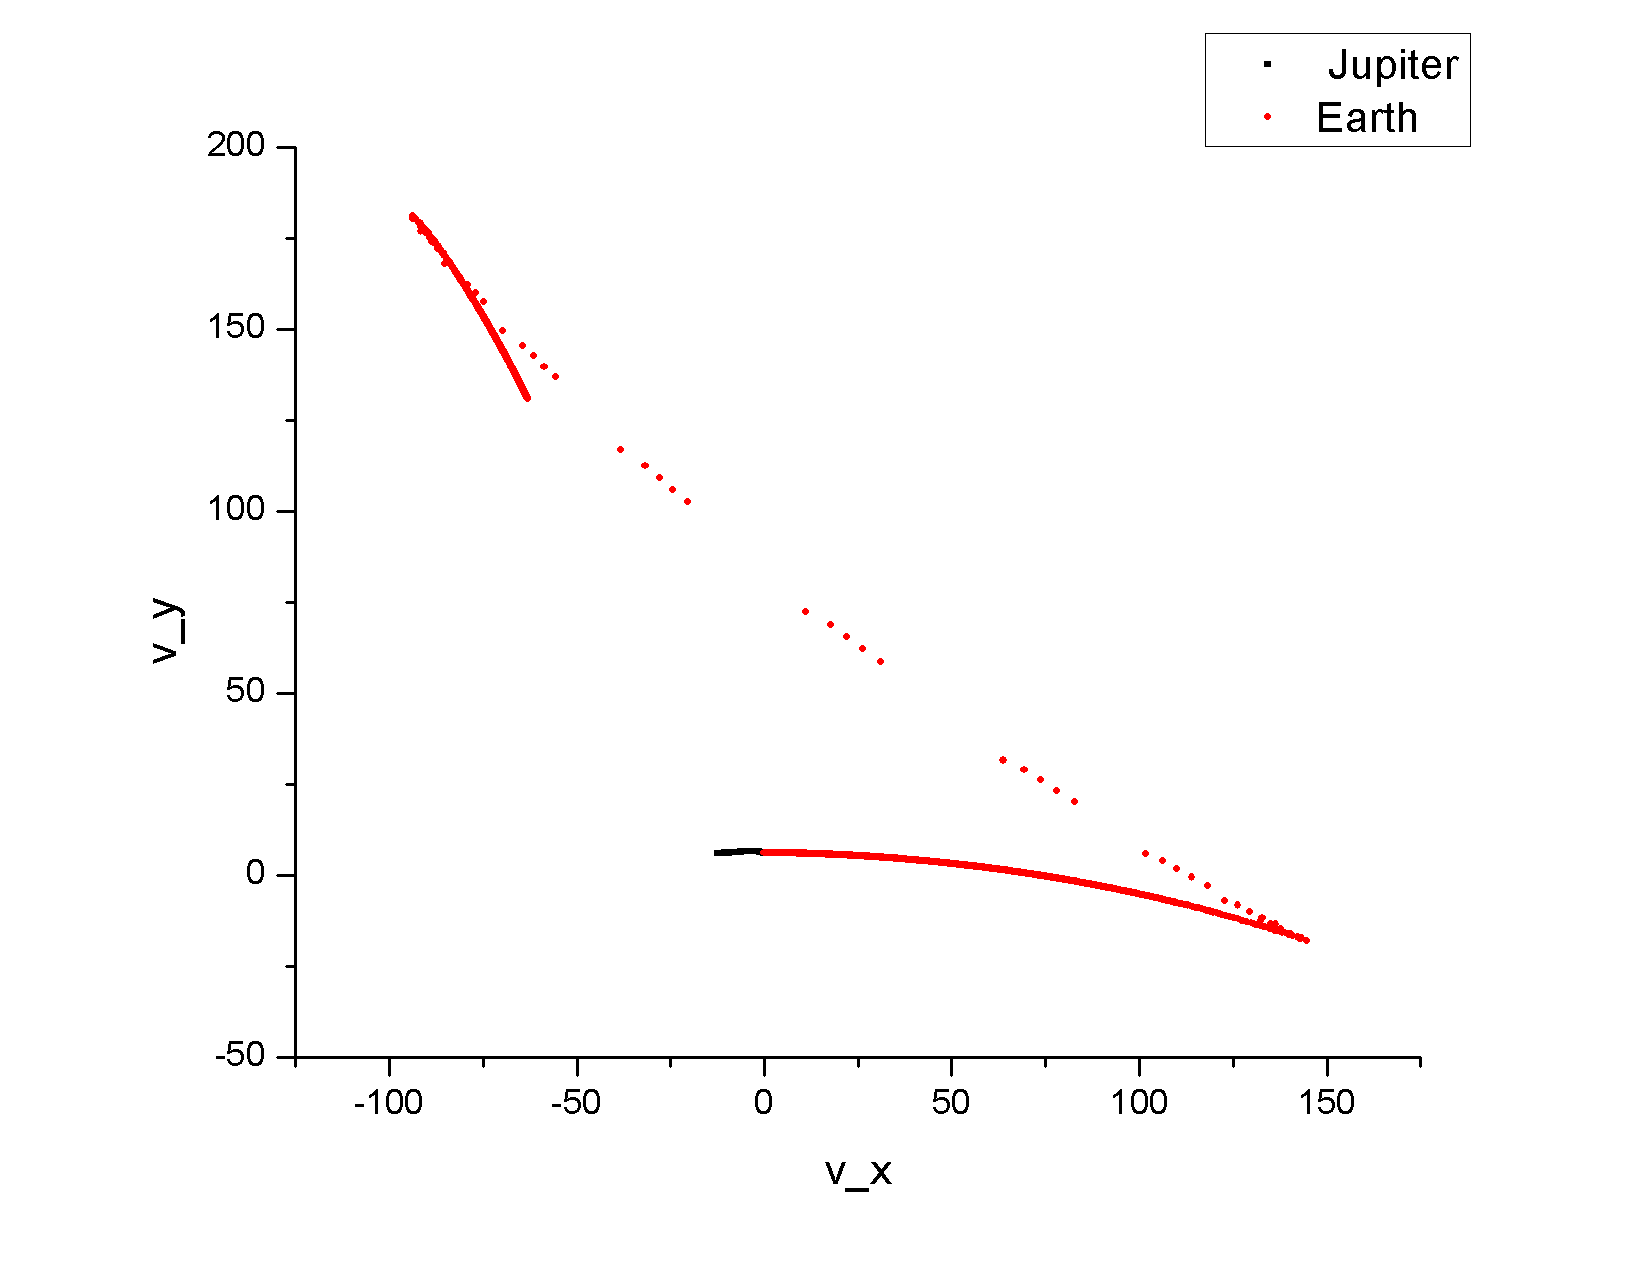
\includegraphics[width=0.75\textwidth]{3testjupitervtav}
\caption{A Jupiter és a Föld sebességének alakulása}
\end{figure}

\begin{figure}[H]
  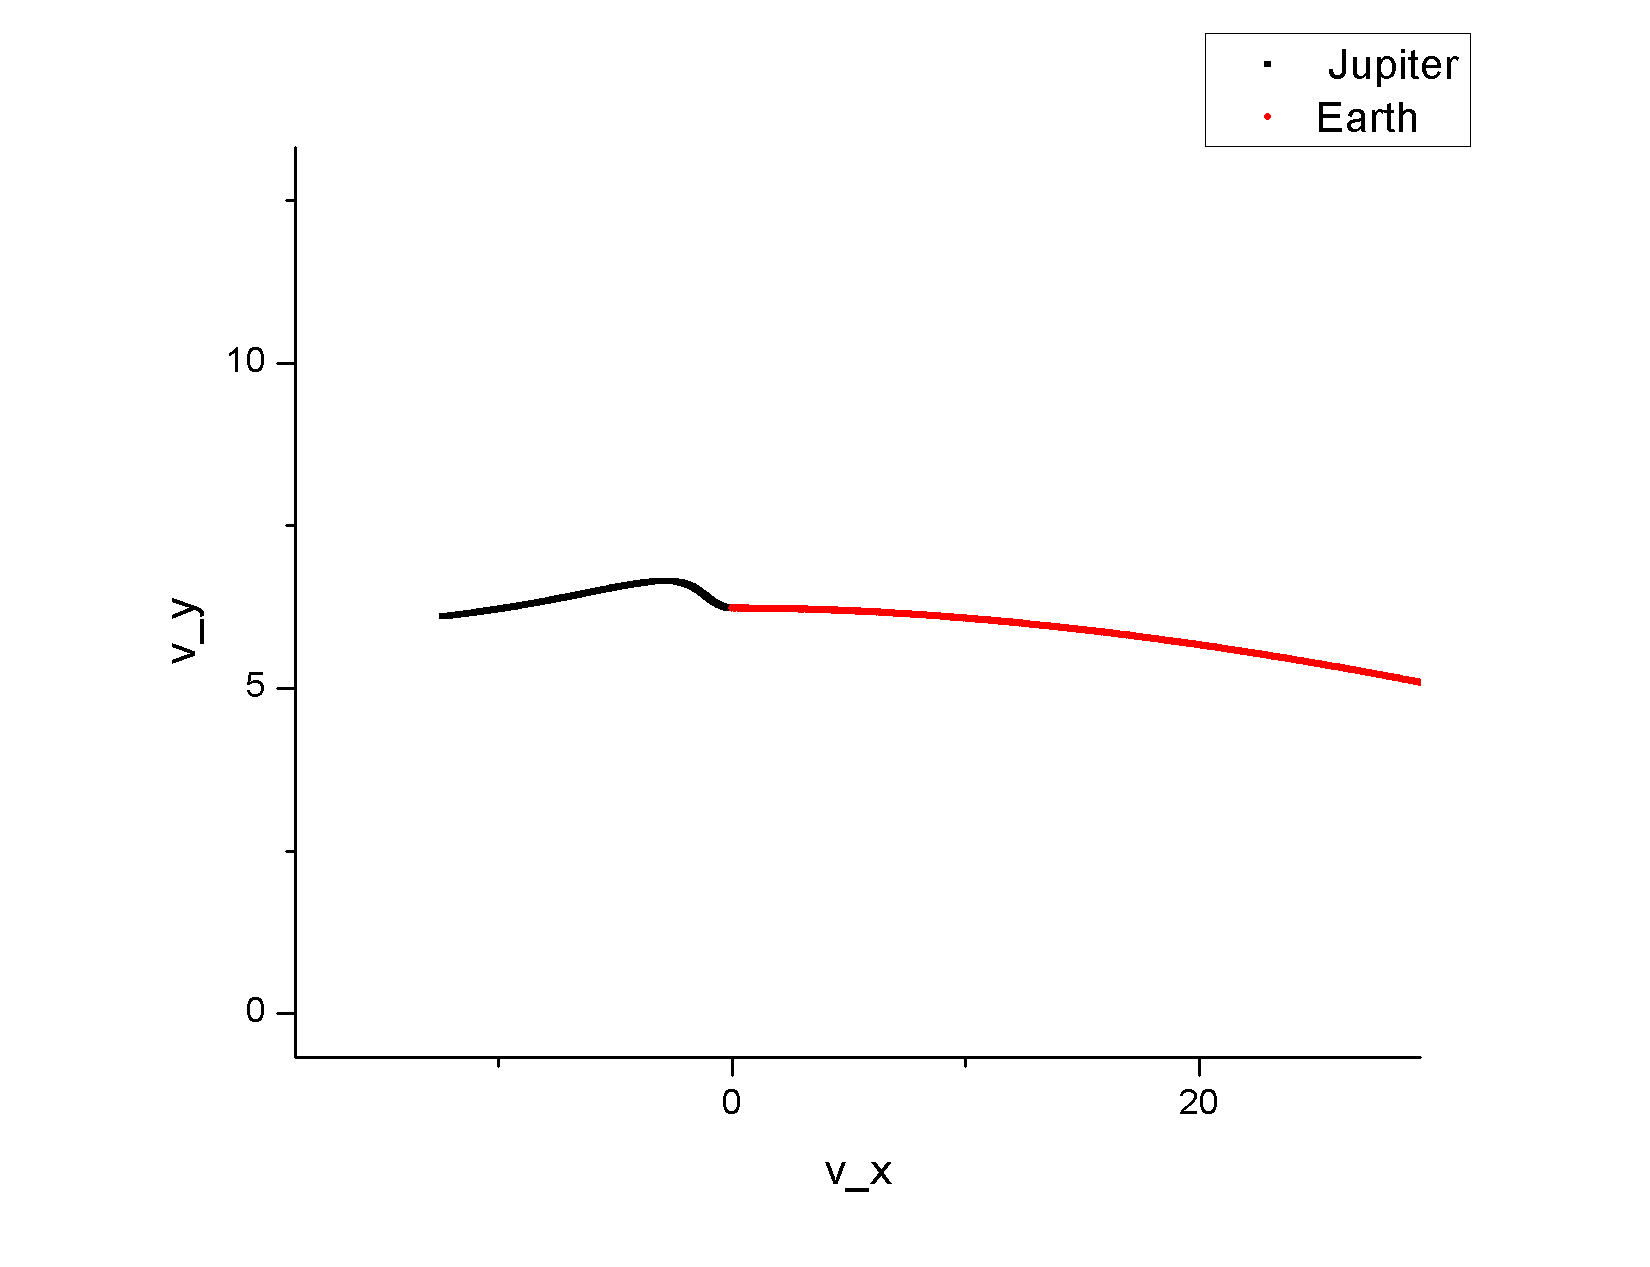
\includegraphics[width=0.75\textwidth]{3testjupiterv}
\caption{A Jupiter és a Föld sebességének alakulása a 0 körül}
\end{figure}





\newpage
\section{Függelék}
\subsection{Három test probléma kód}

\begin{verbatim}
#include <cmath>
#include <cstdlib>
#include <fstream>
#include <iostream>
using namespace std;

#include "vector.hpp"
#include "odeint.hpp"
using namespace cpl;

const double pi = 4 * atan(1.0);
const double GmPlusM = 4 * pi * pi;

bool switch_t_with_y = false;    //  to interpolate to y = 0

//  1. testre az egyenlet
Vector f(const Vector& x) {
    double t = x[0], r_x = x[1], r_y = x[2], v_x = x[3], v_y = x[4], r_x2=x[5], r_y2=x[6], mass=x[9], mass2=x[10];
    double rSquared = r_x*r_x + r_y*r_y;
    double rCubed = rSquared * sqrt(rSquared);
    double rSquared2 = (r_x-r_x2)*(r_x-r_x2) + (r_y-r_y2)*(r_y-r_y2);
    double rCubed2 = rSquared2 * sqrt(rSquared2);
    Vector f(5);
    f[0] = 1;
    f[1] = v_x;
    f[2] = v_y;
    f[3] = - GmPlusM * r_x / rCubed- GmPlusM *mass2* (r_x-r_x2) / rCubed2;
    f[4] = - GmPlusM * r_y / rCubed- GmPlusM *mass2* (r_y-r_y2) / rCubed2;
    if (switch_t_with_y) {
        //  use y as independent variable
        for (int i = 0; i < 5; i++)
            f[i] /= v_y;
    }
    return f;
}
//  2. testre az egyenlet
Vector g(const Vector& x) {
    double t = x[0], r_x = x[5], r_y = x[6], v_x = x[7], v_y = x[8], r_x2=x[1], r_y2=x[2], mass=x[9], mass2=x[10];
    double rSquared = r_x*r_x + r_y*r_y;
    double rCubed = rSquared * sqrt(rSquared);
    double rSquared2 = (r_x-r_x2)*(r_x-r_x2) + (r_y-r_y2)*(r_y-r_y2);
    double rCubed2 = rSquared2 * sqrt(rSquared2);
    Vector g(5);
    g[0] = 1;
    g[1] = v_x;
    g[2] = v_y;
    g[3] = - GmPlusM * r_x / rCubed- GmPlusM *mass* (r_x-r_x2) / rCubed2;
    g[4] = - GmPlusM * r_y / rCubed- GmPlusM *mass* (r_y-r_y2) / rCubed2;
    if (switch_t_with_y) {
        //  use y as independent variable
        for (int i = 0; i < 5; i++)
            g[i] /= v_y;
    }
    return g;
}

//  Change independent variable from t to y and step back to y = 0
void interpolate_crossing(Vector x, int& crossing) {
    ++crossing;
    switch_t_with_y = true;
    RK4Step(x, -x[2], f);
    cout << " crossing " << crossing << "\t t = " << x[0]
         << "\t x = " << x[1] << endl;
    switch_t_with_y = false;
}

int main() {
    cout << " Kepler orbit comparing fixed and adaptive Runge-Kutta\n"
         << " -----------------------------------------------------\n"
         << " Enter aphelion distance in AU, and eccentricity and mass: ";
    double r_ap, eccentricity, a, T, v0, m;
    cin >> r_ap >> eccentricity >> m;
    a = r_ap / (1 + eccentricity);
    T = pow(a, 1.5);
    v0 = sqrt(GmPlusM * (2 / r_ap - 1 / a));
    cout << " Enter number of periods, step size, and adaptive accuracy: ";
    double periods, dt, accuracy;
    cin >> periods >> dt >> accuracy;
    cout<< "bonus body dist and ecc. and mass:";
    double x2, y2, v02, a2, m2;
    cin >> x2 >> y2>> m2;
    a2 = x2 / (1 + y2);
    v02 = sqrt(GmPlusM * (2 / r_ap - 1 / a2));
    Vector x0(11);
    x0[0] = 0;  x0[1] = r_ap;  x0[2] = 0;  x0[3] = 0;  x0[4] = v0; 
    x0[5] = x2; x0[6] = 0; x0[7] =0; x0[8] = v02; x0[9] = m; x0[10] = m2;

    ofstream dataFile("fixed.data");
    Vector x = x0;
    Vector y =x0;
    int steps = 0, crossing = 0;
    cout << "\n Integrating with fixed step size" << endl;
    do {
        for (int i = 0; i < 5; i++)
            dataFile << x[i] << '\t';
        for (int i = 1; i < 5; i++)
            dataFile << y[i] << '\t';
        double q = x[2];
         double w = y[2];
        dataFile<<endl;
        RK4Step(x, dt, f);
        RK4Step(y, dt, g);
        ++steps;
        if (q * x[2] < 0)
            interpolate_crossing(x, crossing);
        if (w * y[2] < 0)
            interpolate_crossing(y, crossing);
    } while (x[0] < periods * T);
    cout << " number of fixed size steps = " << steps << endl;
    cout << " data in file fixed.data" << endl;
    dataFile.close();


}
\end{verbatim}






\newpage


\begin{thebibliography}{2}

 
\bibitem{jegyzet} 
Jegyzet
\\\texttt{$https://stegerjozsef.web.elte.hu/teaching/szamszim/bolygo.pdf$}
 
\bibitem{forraskod} 
Forráskód
\\\texttt{$https://stegerjozsef.web.elte.hu/teaching/szamszim/kepler.tgz$}

\bibitem{wiki} 
3 test
\\\texttt{$https://en.wikipedia.org/wiki/Three-body_problem$}

\bibitem{wiki} 
Lagrange pontok
\\\texttt{$https://en.wikipedia.org/wiki/Lagrangian_point$}

\end{thebibliography}













\end{document}

